\section{\texorpdfstring{\emph{How an Ancient Algorithm and a Family Tree of Right Triangles Turned Out to Be the Same Thing}}{How an Ancient Algorithm and a Family Tree of Right Triangles Turned Out to Be the Same Thing}}\label{ch2-how-an-ancient-algorithm-and-a-family-tree-of-right-triangles-turned-out-to-be-the-same-thing}



\section{The Puzzle of the Perfect Triangle Factory}\label{ch2-the-puzzle-of-the-perfect-triangle-factory}

Suppose you own a factory that manufactures right triangles with whole-number sides. Business is good --- there is an infinite market for \index{Pythagorean triple}Pythagorean triples, as we proved in the last chapter --- but your operation is modest. Your supplier has given you exactly one triangle to start: the humble \((3, 4, 5)\). Or rather, since we found it convenient last time to work with Euclid's parameters, your seed is the pair \((m, n) = (2, 1)\), which produces \(a = m^2 - n^2 = 3\), \(b = 2mn = 4\), \(c = m^2 + n^2 = 5\).

Your factory floor contains exactly two machines. They are bolted to the concrete, humming faintly, each with a slot for an input card and a slot for an output card. The input card holds a pair of integers \((m, n)\). The output card holds a new pair. The machines are labeled \(\mathbf{M}_1\) and \(\mathbf{M}_3\), and they operate by the following recipes:

\begin{itemize}

\item
  \textbf{Machine \(\mathbf{M}_1\):} Feed in \((m, n)\). Out comes \((2m - n,\; m)\).
\item
  \textbf{Machine \(\mathbf{M}_3\):} Feed in \((m, n)\). Out comes \((m + 2n,\; n)\).
\end{itemize}

That is all. Two machines, two recipes, one seed. Here is my puzzle, and I encourage you to grab a pencil before reading further:

\begin{quote}
\emph{Can these two machines --- and nothing else --- manufacture every primitive Pythagorean triple that will ever exist?}
\end{quote}

Let us fire up the assembly line. Start with the seed \((2, 1)\):

\begin{itemize}

\item
  Feed \((2, 1)\) into \(\mathbf{M}_1\): out comes \((2 \cdot 2 - 1,\; 2) = (3, 2)\).
\item
  Feed \((2, 1)\) into \(\mathbf{M}_3\): out comes \((2 + 2 \cdot 1,\; 1) = (4, 1)\).
\end{itemize}

Two new pairs. Now feed each of \emph{those} into both machines:

\begin{itemize}

\item
  \(\mathbf{M}_1(3, 2) = (4, 3)\), giving the triple \((7, 24, 25)\).
\item
  \(\mathbf{M}_3(3, 2) = (7, 2)\), giving the triple \((45, 28, 53)\).
\item
  \(\mathbf{M}_1(4, 1) = (7, 4)\), giving the triple \((33, 56, 65)\).
\item
  \(\mathbf{M}_3(4, 1) = (6, 1)\), giving the triple \((35, 12, 37)\).
\end{itemize}

Already the tree is branching. Two children at each node, four grandchildren, eight great-grandchildren, and so on, the family growing without bound. Convert each \((m, n)\) pair back to a Pythagorean triple using Euclid's formulas --- \(a = m^2 - n^2\), \(b = 2mn\), \(c = m^2 + n^2\) --- and you have a genealogical chart of right triangles.


\begin{figure}[htbp]
\centering
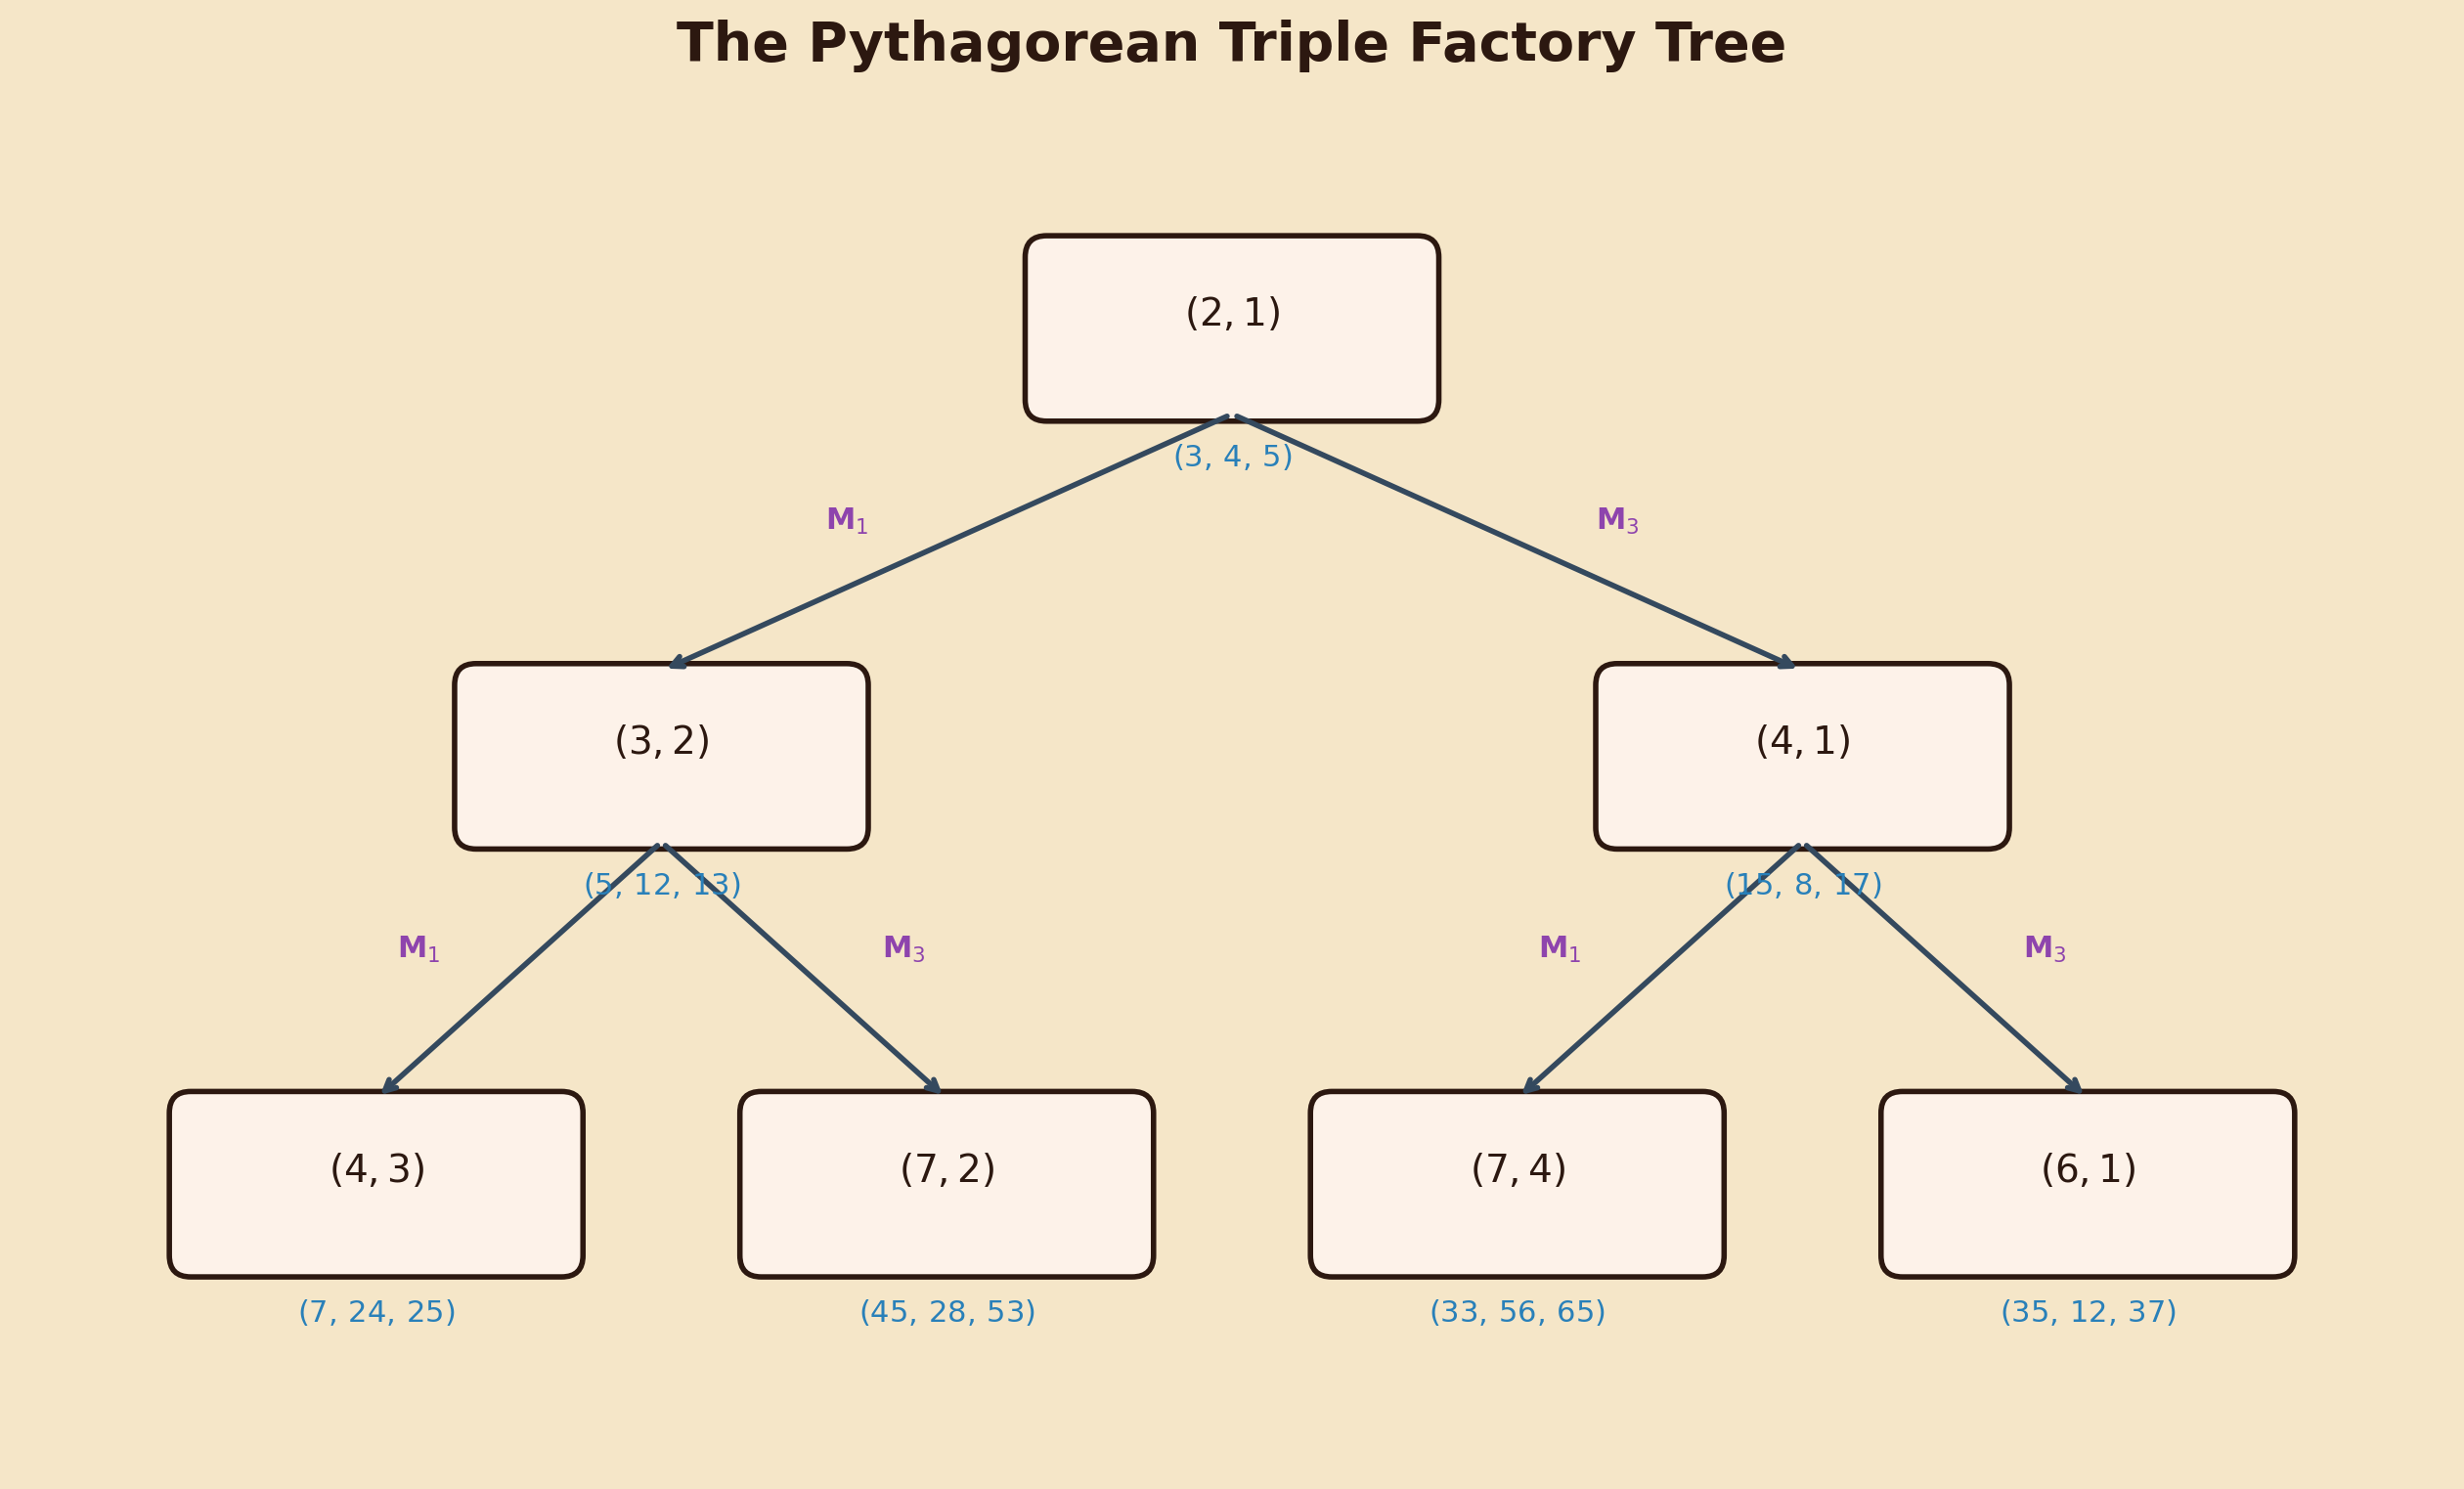
\includegraphics[width=0.82\textwidth]{../Chapter2/images/fig01_factory_tree.png}
\end{figure}


The answer to the puzzle --- and it is a remarkable fact --- is \emph{yes}. Every primitive Pythagorean triple appears somewhere in this tree, exactly once. No duplicates, no omissions. The machines are complete and non-redundant.

For readers of the last chapter, this claim may ring a bell. There we met the \index{Berggren tree}Berggren tree in its \(3 \times 3\) incarnation --- three matrices \(\mathbf{A}\), \(\mathbf{B}\), \(\mathbf{C}\) acting on triples \((a, b, c)\) directly. What we are seeing now is the same tree in disguise, compressed into the \(2 \times 2\) world of Euclid's parameters. The full Berggren tree has three branches at each node; our parameter tree has two, because we have factored out the symmetry that swaps the legs \(a\) and \(b\). (Swapping legs corresponds to swapping \(m^2 - n^2\) and \(2mn\), which is a bookkeeping choice, not a genuinely new triangle.) The mathematical content is identical --- we have merely changed the lens.

The two machines, if you insist on writing them as matrices acting on column vectors \(\begin{pmatrix} m \\ n \end{pmatrix}\), are:

\[
\mathbf{M}_1 = \begin{pmatrix} 2 & -1 \\ 1 & 0 \end{pmatrix}, \qquad
\mathbf{M}_3 = \begin{pmatrix} 1 & 2 \\ 0 & 1 \end{pmatrix}.
\]

But for now, think of them as recipes, not as arrays of numbers. The matrix notation is simply a compact way of saying ``do \emph{this} to \(m\) and \emph{that} to \(n\).''

A capsule of history is in order. The man who first saw this tree was Berggren --- B. Berggren, a Swedish schoolteacher who published his discovery in 1934 in a journal so obscure that the mathematical world barely noticed. His paper, written in Swedish, proved that three \(3 \times 3\) matrices generate every primitive Pythagorean triple from \((3, 4, 5)\). It was one of the most quietly influential results in number theory: a complete, constructive enumeration of an infinite set, hiding in plain sight. Decades passed before the result was rediscovered independently by Hall (1970) and later by Barning. Today it is a staple of recreational mathematics --- but Berggren himself, as far as anyone knows, never learned how famous his tree would become.



\section{Why the Machines Never Jam}\label{ch2-why-the-machines-never-jam}

Here is a worry that might have crossed your mind during the factory tour. Suppose a customer brings back a triangle and demands to know its \emph{parent} --- the triangle that produced it. Can you always trace a triple back through the tree to the root? In other words, can the factory be run in reverse?

The answer hinges on a single number: the \emph{determinant} of each machine. Compute:

\[
\det(\mathbf{M}_1) = (2)(0) - (-1)(1) = 0 + 1 = 1.
\]

\[
\det(\mathbf{M}_3) = (1)(1) - (2)(0) = 1 - 0 = 1.
\]

Both determinants equal one. This is not a coincidence --- it is the whole point.

A \(2 \times 2\) matrix with integer entries and determinant \(1\) belongs to a distinguished club called the \emph{special linear group}, denoted \(\mathrm{SL}(2, \mathbb{Z})\). The members of this club have a superpower: they are always invertible \emph{over the integers}. That is, if \(\mathbf{M}\) is in \(\mathrm{SL}(2, \mathbb{Z})\), then there exists another matrix \(\mathbf{M}^{-1}\), also with integer entries and determinant \(1\), such that \(\mathbf{M} \cdot \mathbf{M}^{-1} = \mathbf{I}\), the identity matrix. No fractions, no rounding, no approximation. Every step can be perfectly undone.

Think of it this way. The integer lattice \(\mathbb{Z}^2\) is an infinite grid of dots, one at every point with whole-number coordinates. A matrix in \(\mathrm{SL}(2, \mathbb{Z})\) reshapes this grid --- it can shear it, rotate it, stretch it in one direction and compress it in another --- but it never tears it, never folds it, and never creates or destroys any dots. The area of every fundamental parallelogram remains exactly \(1\). This is what ``determinant one'' means geometrically: the transformation preserves area perfectly.

The inverse machines are:

\[
\mathbf{M}_1^{-1} = \begin{pmatrix} 0 & 1 \\ -1 & 2 \end{pmatrix}, \qquad
\mathbf{M}_3^{-1} = \begin{pmatrix} 1 & -2 \\ 0 & 1 \end{pmatrix}.
\]

You can verify these by direct multiplication --- a satisfying exercise I recommend doing at least once. For \(\mathbf{M}_1\):

\[
\mathbf{M}_1 \cdot \mathbf{M}_1^{-1} = \begin{pmatrix} 2 & -1 \\ 1 & 0 \end{pmatrix} \begin{pmatrix} 0 & 1 \\ -1 & 2 \end{pmatrix} = \begin{pmatrix} (0+1) & (2-2) \\ (0+0) & (1+0) \end{pmatrix} = \begin{pmatrix} 1 & 0 \\ 0 & 1 \end{pmatrix}. \quad \checkmark
\]

And for \(\mathbf{M}_3\):

\[
\mathbf{M}_3 \cdot \mathbf{M}_3^{-1} = \begin{pmatrix} 1 & 2 \\ 0 & 1 \end{pmatrix} \begin{pmatrix} 1 & -2 \\ 0 & 1 \end{pmatrix} = \begin{pmatrix} 1 & 0 \\ 0 & 1 \end{pmatrix}. \quad \checkmark
\]

The factory runs backward without a hitch. Feed any triple into the inverse machines, and you can trace its ancestry all the way back to \((2, 1)\).


\begin{figure}[htbp]
\centering
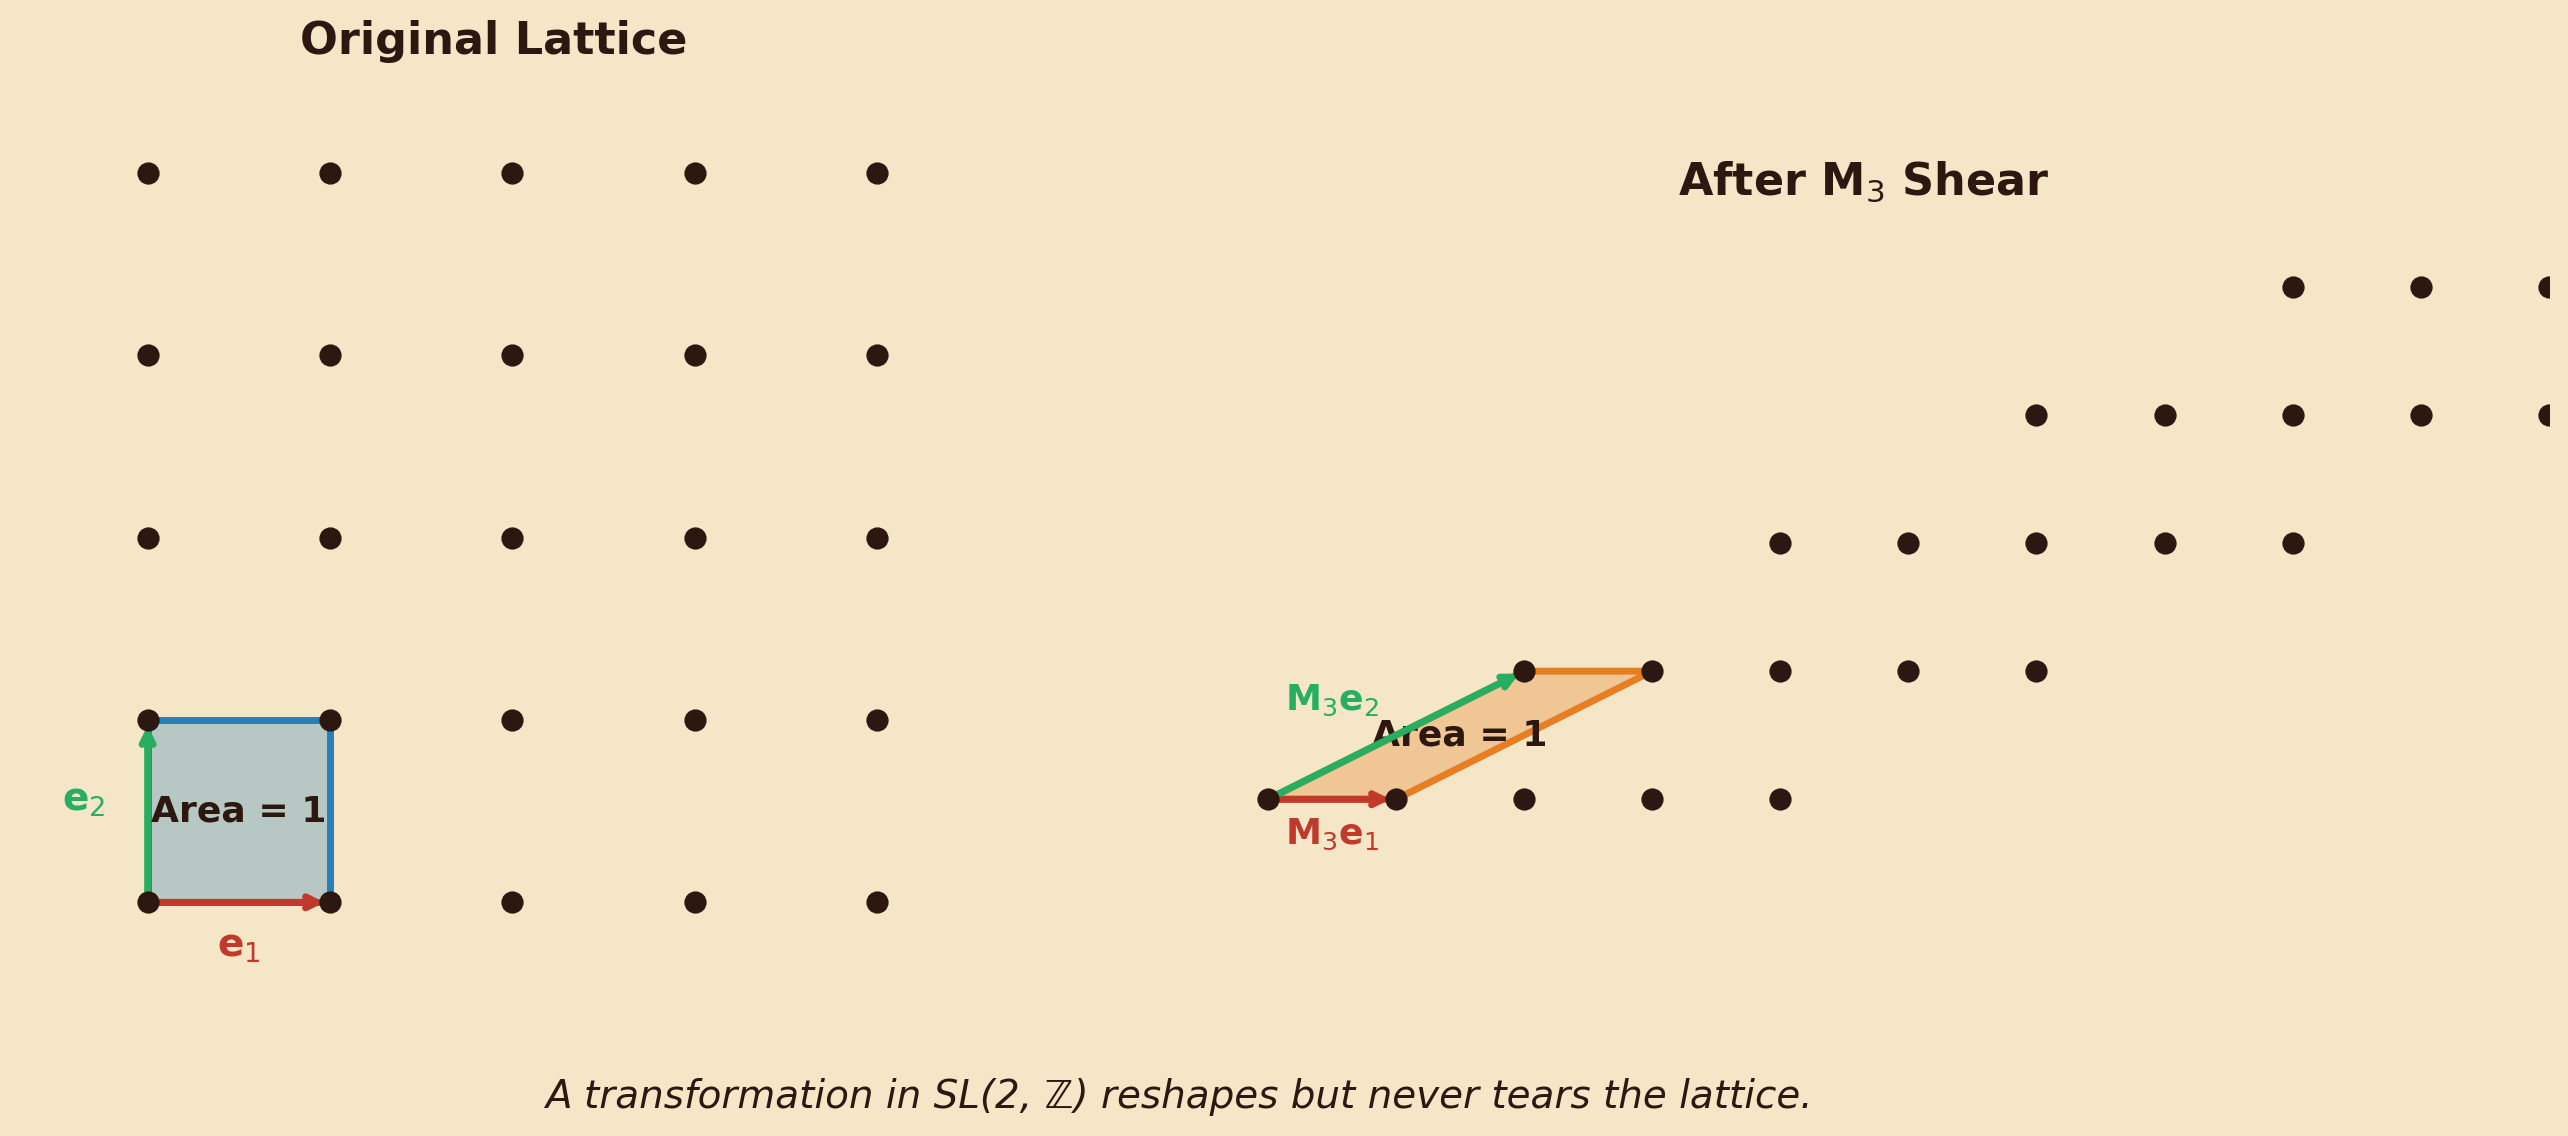
\includegraphics[width=0.82\textwidth]{../Chapter2/images/fig02_lattice_shear.png}
\end{figure}


The group \(\mathrm{SL}(2, \mathbb{Z})\) has a long and glamorous history quite apart from Pythagorean triples. It is the symmetry group of the \emph{modular surface} --- a strange, infinite, self-similar landscape that tiles the upper half of the complex plane. If you have ever seen one of M. C. Escher's hyperbolic tilings --- those dizzying patterns of interlocking fish or angels-and-devils that grow ever finer as they approach a bounding circle --- you have seen \(\mathrm{SL}(2, \mathbb{Z})\) at work. The same group that governs our triangle factory also governs the geometry of modular forms, \index{elliptic curves}elliptic curves, and the deep symmetries of number theory. Martin Gardner, who adored Escher, would have been delighted by the connection. We shall return to it later in the book; for now, it is enough to know that our two humble machines belong to a very distinguished family.



\section{Euclid's Oldest Algorithm Gets a Makeover}\label{ch2-euclids-oldest-algorithm-gets-a-makeover}

Here is a party trick that is at least 2,300 years old. Think of two positive integers --- say, \(m = 17\) and \(n = 5\). Now play the following game:

\begin{enumerate}
\def\labelenumi{\arabic{enumi}.}

\item
  Divide the larger by the smaller. Write down the quotient. Replace the larger number with the remainder.
\item
  Repeat until the remainder is zero.
\item
  The last nonzero remainder is the greatest common divisor.
\end{enumerate}

For \(17\) and \(5\):

\[
17 = 3 \cdot 5 + 2 \qquad (\text{quotient } 3, \text{ remainder } 2)
\] \[
5 = 2 \cdot 2 + 1 \qquad (\text{quotient } 2, \text{ remainder } 1)
\] \[
2 = 2 \cdot 1 + 0 \qquad (\text{quotient } 2, \text{ remainder } 0)
\]

The last nonzero remainder is \(1\), so \(\gcd(17, 5) = 1\). The numbers are coprime.

This is the \emph{Euclidean algorithm}, described in Book VII of Euclid's \emph{Elements} around 300 BCE --- though it was almost certainly known to earlier Greek mathematicians, and some scholars suspect the Babylonians had a version of it. Donald Knuth, in \emph{The Art of Computer Programming}, called it ``the granddaddy of all algorithms,'' and with good reason: it is arguably the oldest nontrivial algorithm still in daily use, running inside every computer that performs modular arithmetic, every cryptographic protocol that computes key exchanges, every calculator that simplifies fractions.

But here is the secret nobody tells you at the party: every single step of this game can be written as multiplication by a tiny \(2 \times 2\) matrix.

Define the \emph{quotient matrix} for quotient \(q\):

\[
\mathbf{Q}(q) = \begin{pmatrix} 0 & 1 \\ 1 & -q \end{pmatrix}.
\]

Watch what happens when you multiply this matrix by the column vector \(\begin{pmatrix} a \\ b \end{pmatrix}\), where \(a = q \cdot b + r\):

\[
\mathbf{Q}(q) \begin{pmatrix} a \\ b \end{pmatrix} = \begin{pmatrix} 0 \cdot a + 1 \cdot b \\ 1 \cdot a + (-q) \cdot b \end{pmatrix} = \begin{pmatrix} b \\ a - qb \end{pmatrix} = \begin{pmatrix} b \\ r \end{pmatrix}.
\]

The matrix swaps the two numbers and replaces the larger one with the remainder. That is precisely one step of the Euclidean algorithm. The entire computation on \((17, 5)\) becomes a chain of matrix multiplications:

\[
\begin{pmatrix} 17 \\ 5 \end{pmatrix} \xrightarrow{\mathbf{Q}(3)} \begin{pmatrix} 5 \\ 2 \end{pmatrix} \xrightarrow{\mathbf{Q}(2)} \begin{pmatrix} 2 \\ 1 \end{pmatrix} \xrightarrow{\mathbf{Q}(2)} \begin{pmatrix} 1 \\ 0 \end{pmatrix}.
\]

Or, if you prefer a single equation:

\[
\mathbf{Q}(2) \cdot \mathbf{Q}(2) \cdot \mathbf{Q}(3) \begin{pmatrix} 17 \\ 5 \end{pmatrix} = \begin{pmatrix} 1 \\ 0 \end{pmatrix}.
\]


\begin{figure}[htbp]
\centering
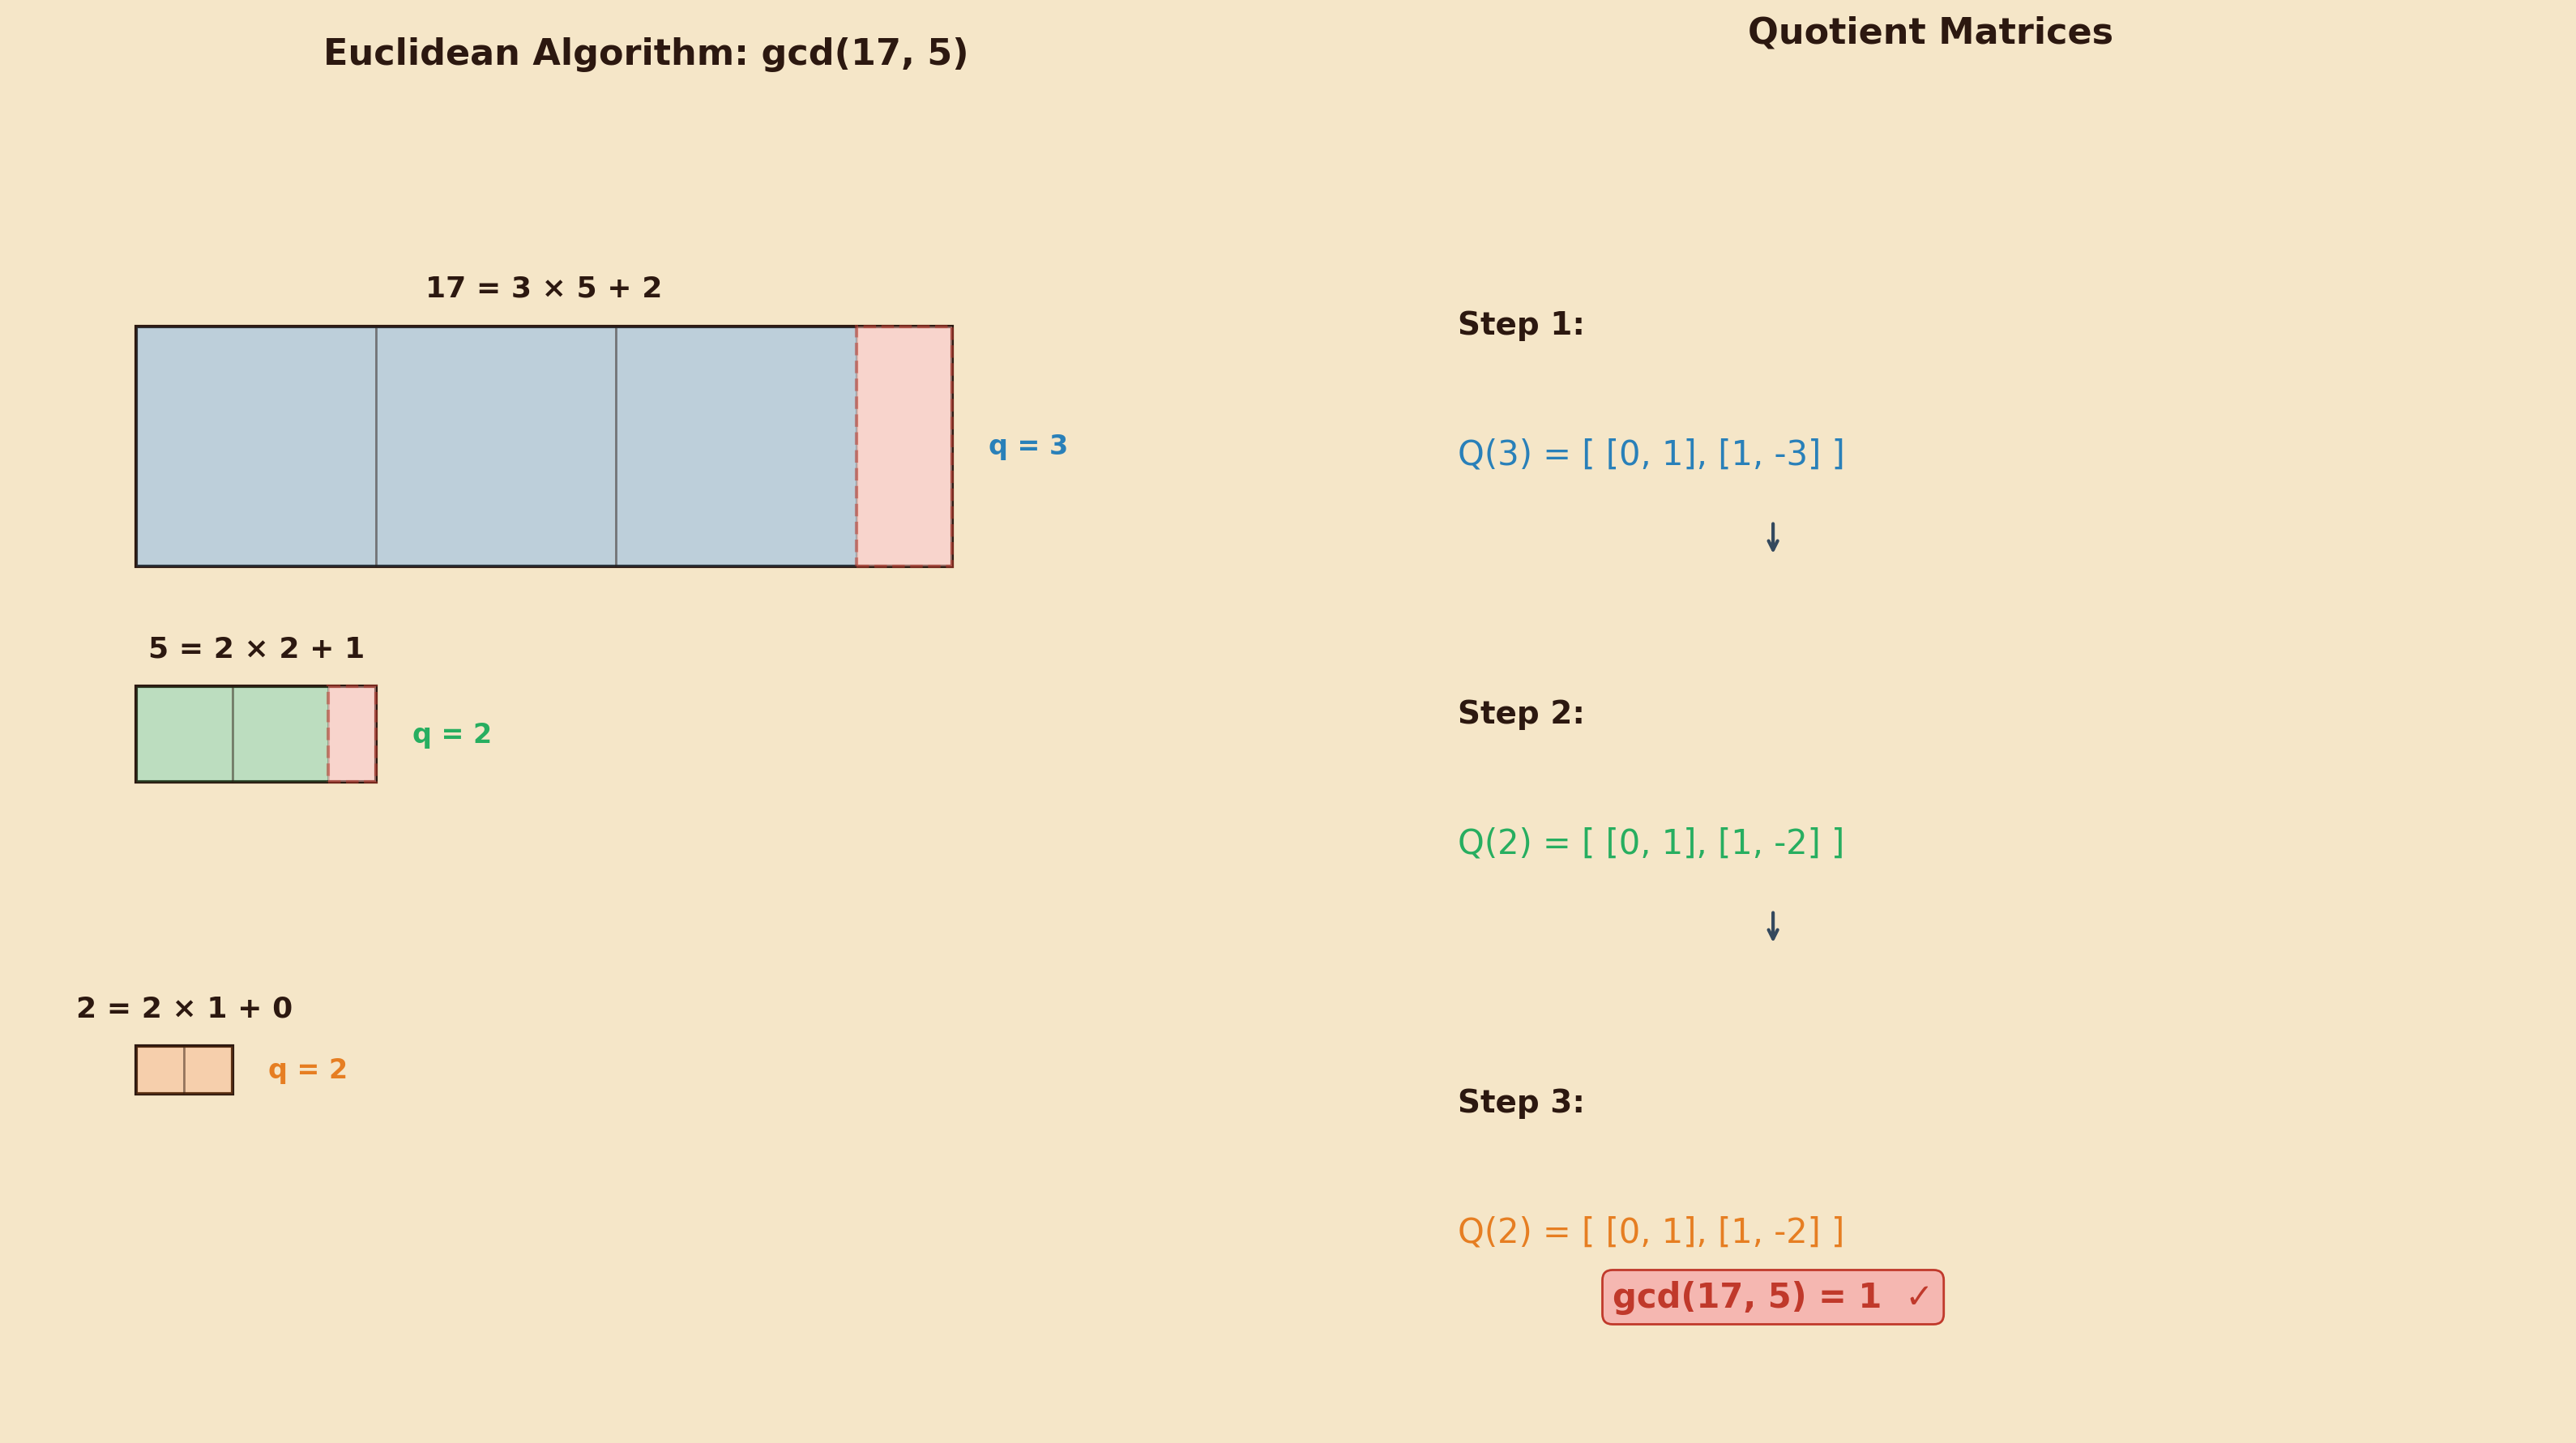
\includegraphics[width=0.82\textwidth]{../Chapter2/images/fig03_euclid_staircase.png}
\end{figure}


There is a delicious detail hiding in the determinants. Compute:

\[
\det \mathbf{Q}(q) = (0)(- q) - (1)(1) = -1.
\]

The determinant is \(-1\), regardless of \(q\). Every step of the Euclidean algorithm \emph{flips the orientation} of the plane. Two steps flip it back. Three flip it again. This alternating sign is not a mere curiosity --- it is the heartbeat of continued fractions. The sequence of quotients \([3; 2, 2]\) that we extracted from the pair \((17, 5)\) is exactly the continued fraction expansion of \(17/5\):

\[
\frac{17}{5} = 3 + \cfrac{1}{2 + \cfrac{1}{2}}.
\]

The alternating signs of the determinants produce the alternating signs in the convergents of a continued fraction --- the numerators overshoot and undershoot the true value in strict alternation, a pattern that Bombelli noticed in 1572 and Wallis formalized in 1655. The Euclidean algorithm, continued fractions, and \(2 \times 2\) matrices are three faces of the same crystal. We are about to discover a fourth.



\section{The Astonishing Coincidence}\label{ch2-the-astonishing-coincidence}

We now arrive at the central revelation of this chapter --- the moment when two mathematical objects, developed centuries apart, in completely different contexts, by people who never heard of each other, turn out to be \emph{the same algorithm in disguise}.

Imagine discovering that the blueprint for a Gothic cathedral, drawn by a master mason in 1230, is identical --- line for line --- to the circuit diagram of a 1990s computer chip. That is roughly the level of surprise we are about to experience.

Recall the inverse machines from the triangle factory:

\[
\mathbf{M}_1^{-1} = \begin{pmatrix} 0 & 1 \\ -1 & 2 \end{pmatrix}, \qquad
\mathbf{M}_3^{-1} = \begin{pmatrix} 1 & -2 \\ 0 & 1 \end{pmatrix}.
\]

Now let us see what each inverse machine does to a generic pair \((m, n)\).

\textbf{Inverse Machine \(\mathbf{M}_3^{-1}\):}

\[
\mathbf{M}_3^{-1} \begin{pmatrix} m \\ n \end{pmatrix} = \begin{pmatrix} 1 & -2 \\ 0 & 1 \end{pmatrix} \begin{pmatrix} m \\ n \end{pmatrix} = \begin{pmatrix} m - 2n \\ n \end{pmatrix}.
\]

Read that result aloud: ``Replace \(m\) with \(m - 2n\); leave \(n\) alone.'' This is \emph{exactly} the Euclidean algorithm's subtraction step --- subtracting the quotient \(q = 2\) times the smaller number from the larger. It is one step of the continued fraction expansion with a fixed quotient of \(2\).

\textbf{Inverse Machine \(\mathbf{M}_1^{-1}\):}

\[
\mathbf{M}_1^{-1} \begin{pmatrix} m \\ n \end{pmatrix} = \begin{pmatrix} 0 & 1 \\ -1 & 2 \end{pmatrix} \begin{pmatrix} m \\ n \end{pmatrix} = \begin{pmatrix} n \\ 2n - m \end{pmatrix}.
\]

This one is subtler. It swaps the roles of \(m\) and \(n\) (putting \(n\) on top), and replaces \(n\) with \(2n - m\). This is precisely the \emph{swap-and-reduce} step: the Euclidean algorithm does this when the remainder \(m - 2n\) would go negative (meaning \(m < 2n\), so the quotient of \(m\) divided by \(n\) is \(1\), and we need to swap before proceeding with quotient \(2\)).

Do you see it? The inverse Berggren machines \emph{are} Euclidean steps. Running the triangle tree in reverse --- tracing a triple's ancestry back to the root --- performs exactly the same computation as the Euclidean algorithm applied to the parameters \(m\) and \(n\).

Let us verify this with a concrete example. Start with the pair \((7, 2)\). This pair gives the Pythagorean triple \((45, 28, 53)\). Now descend the tree to the root:

\textbf{Tree descent:}

\begin{itemize}

\item
  \((7, 2)\): Is \(7 \ge 2 \cdot 2 = 4\)? Yes. Apply \(\mathbf{M}_3^{-1}\): \((7 - 4,\; 2) = (3, 2)\).
\item
  \((3, 2)\): Is \(3 \ge 2 \cdot 2 = 4\)? No.~Apply \(\mathbf{M}_1^{-1}\): \((2,\; 4 - 3) = (2, 1)\).
\end{itemize}

We have reached the root in two steps.

\textbf{Euclidean algorithm on \((7, 2)\):}

\[
7 = 3 \cdot 2 + 1 \qquad (\text{quotient } 3, \text{ remainder } 1)
\] \[
2 = 2 \cdot 1 + 0 \qquad (\text{quotient } 2, \text{ remainder } 0)
\]

The quotients are \(3\) and \(2\). Now, the tree descent used \emph{one} application of \(\mathbf{M}_3^{-1}\) (which subtracts \(2n\), i.e., quotient \(2\)) followed by one application of \(\mathbf{M}_1^{-1}\) (which swaps and subtracts, handling the remaining quotient of \(1\) plus the next quotient of \(2\)). The bookkeeping differs slightly --- the tree descent bundles the Euclidean steps in pairs --- but the underlying computation is identical. The sequence of subtractions, the sequence of remainders, the final arrival at the base pair: all the same.


\begin{figure}[htbp]
\centering
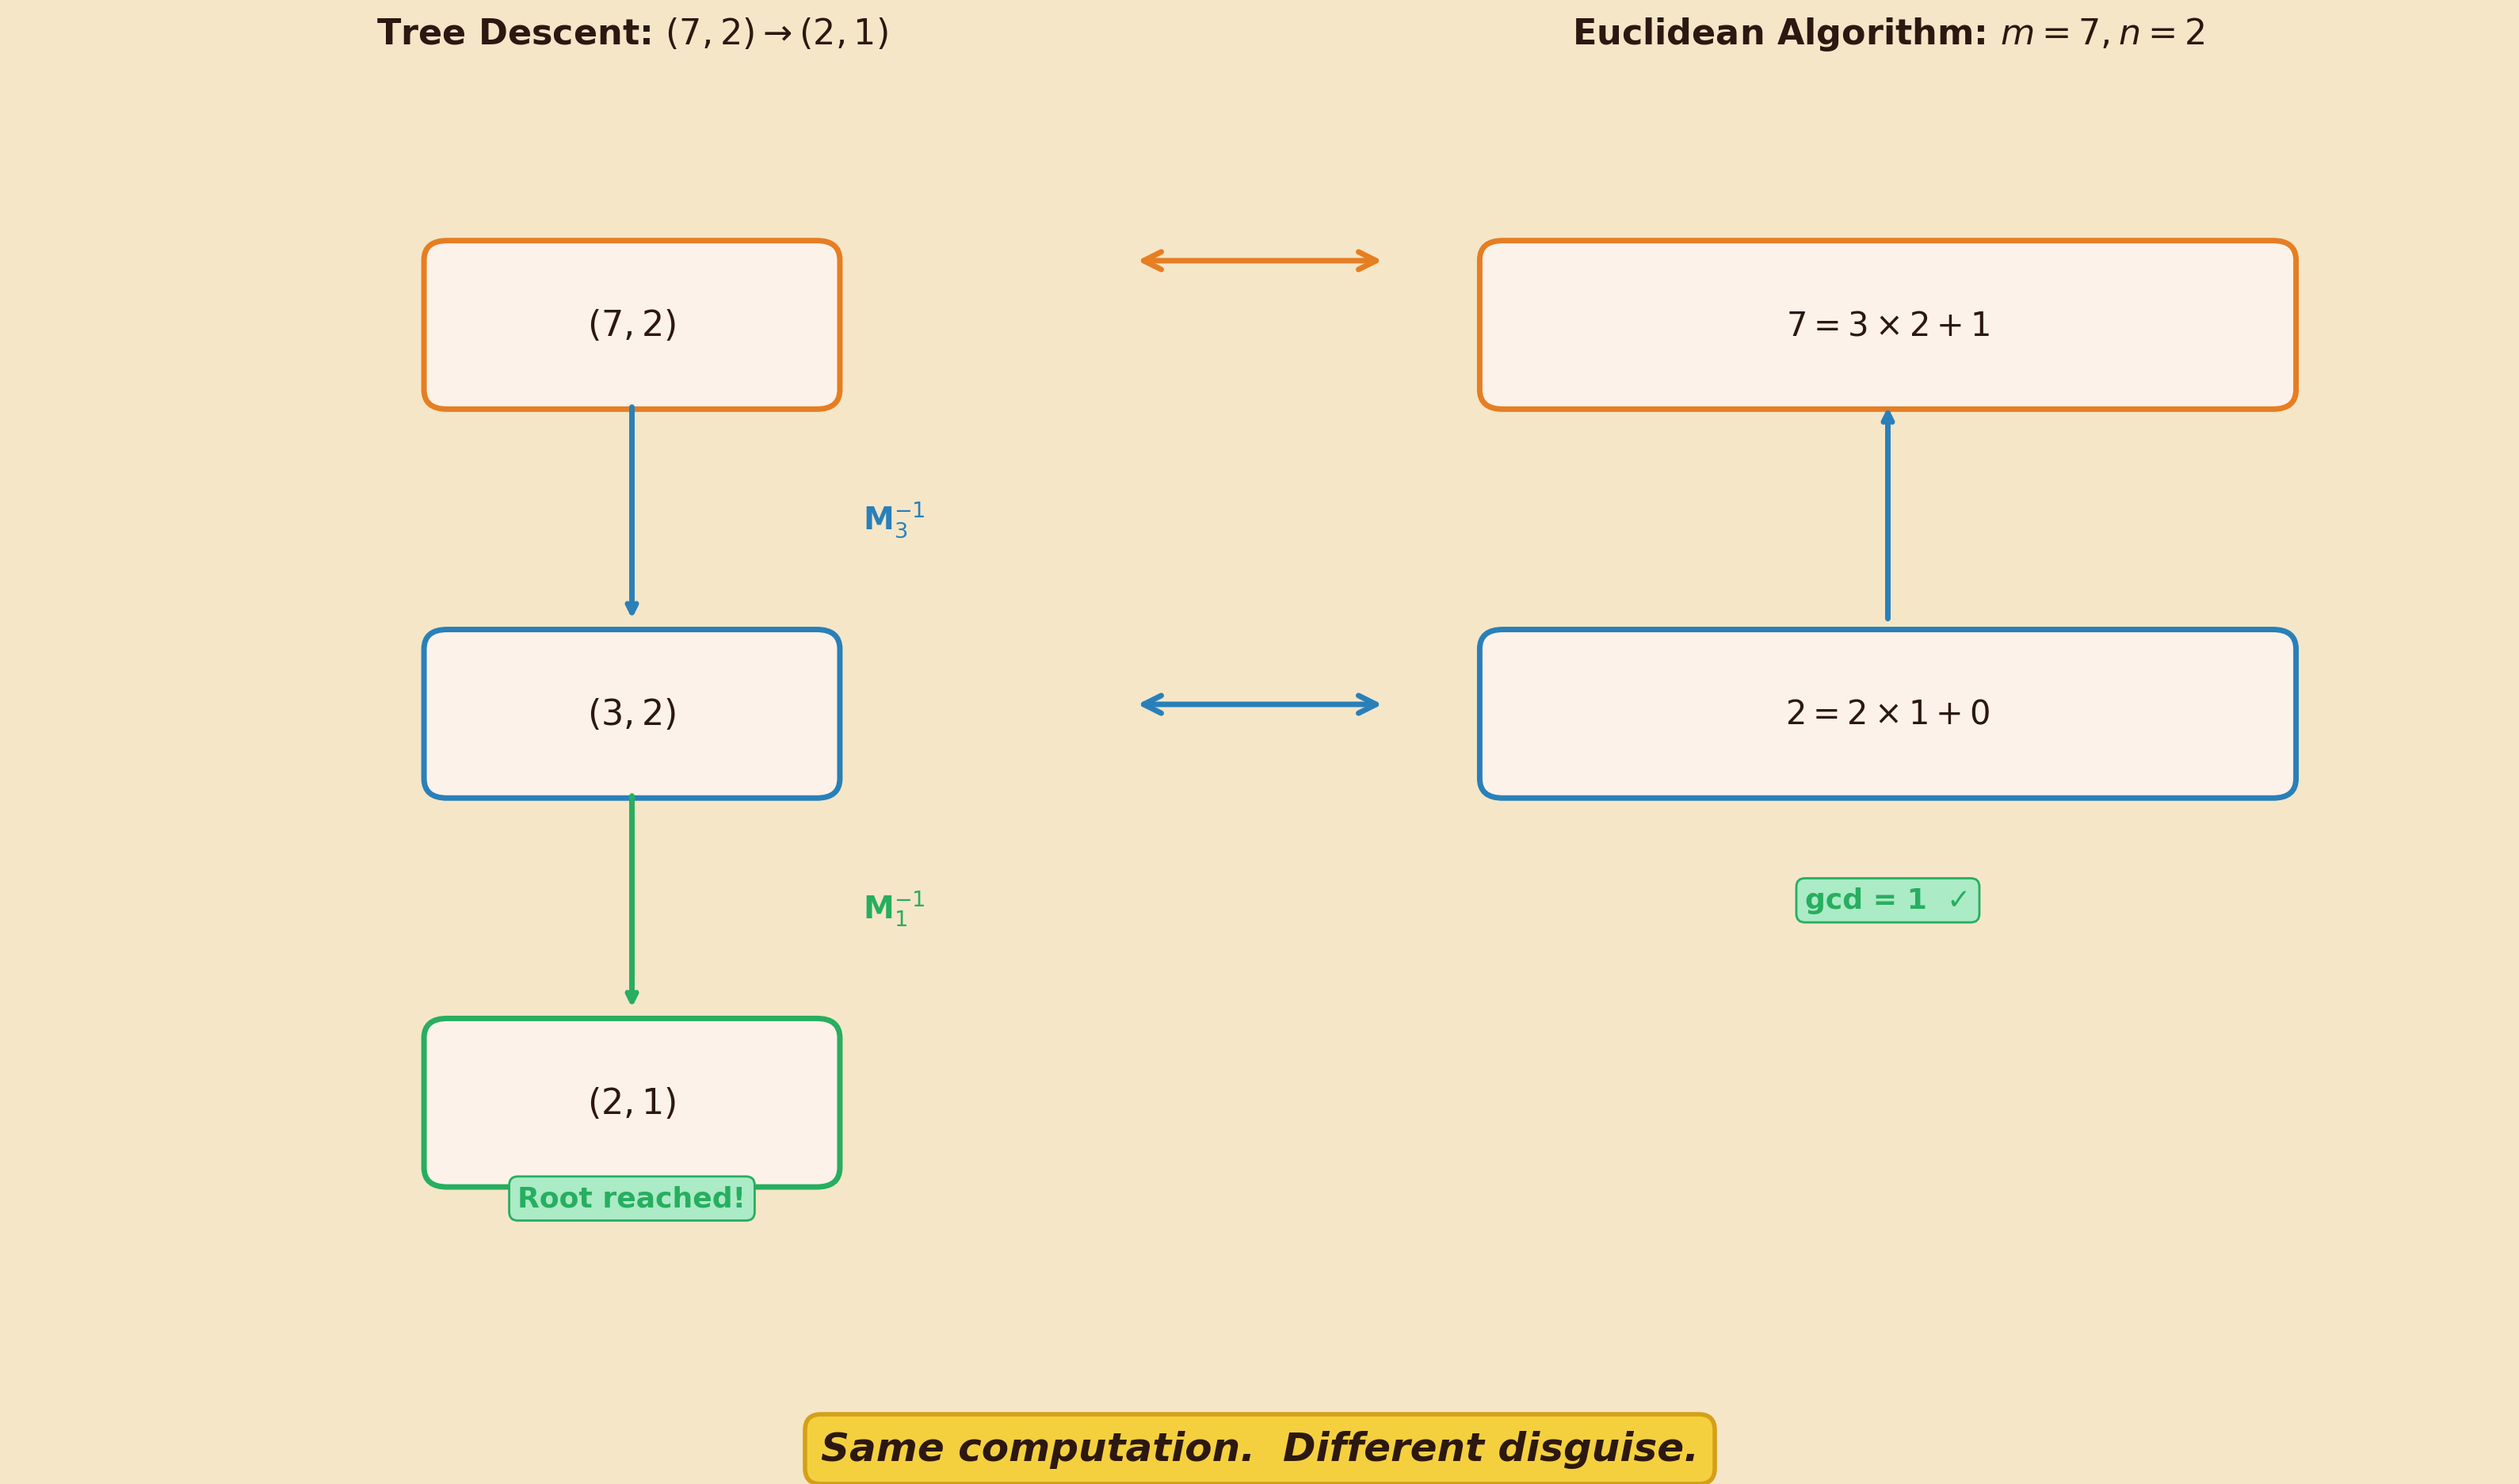
\includegraphics[width=0.82\textwidth]{../Chapter2/images/fig04_tree_vs_euclid.png}
\end{figure}


We can now state the chapter's central theorem --- the \textbf{Lattice-Tree Correspondence} --- in plain language:

\begin{quote}
\textbf{The Lattice-Tree Correspondence.} \emph{Climbing down the Berggren tree --- applying \(\mathbf{M}_3^{-1}\) and \(\mathbf{M}_1^{-1}\) to return to the root --- computes precisely the same sequence of quotients as the Euclidean algorithm applied to the ratio \(m/n\). The tree descent} is \emph{the continued fraction expansion.}
\end{quote}

This is one of those results that, once you see it, seems inevitable --- even \emph{obvious}. Of course the tree descent is the Euclidean algorithm! What else could it be? The matrices are practically the same! And yet, for decades, nobody noticed. Berggren published his tree in 1934. The matrix formulation of the Euclidean algorithm has been known, in one form or another, since at least the nineteenth century. But the explicit connection --- the recognition that the inverse Berggren moves are Euclidean quotient steps --- seems to have gone unremarked until much later.

George Pólya once advised mathematicians to ``look at the problem from the right angle.'' The Lattice-Tree Correspondence is what happens when you finally find that angle. Two constructions that seemed unrelated --- an enumeration of right triangles and an algorithm for greatest common divisors --- snap together like puzzle pieces, because they are governed by the same underlying structure: the arithmetic of \(2 \times 2\) integer matrices with determinant one.



\section{The Speed of Descent}\label{ch2-the-speed-of-descent}

Now that we know the tree descent is the Euclidean algorithm in disguise, we can ask a very practical question: \emph{how fast is it?}

Suppose \(N\) is the product of two secret prime numbers, \(p\) and \(q\), and we are trying to discover them. One approach --- inspired by the factoring bridge from Chapter 1 --- is to search the Berggren tree for a triple whose entries reveal a factor of \(N\). The tree descent gives us a systematic way to do this: start at a carefully chosen node and trace a path back to the root, checking at each step whether the current triple's parameters share a common factor with \(N\).

How many steps will this take? A naïve guess might say ``about \(N\) steps'' --- just try everything. A cleverer guess says ``\(\sqrt{N}\).'' The truth is pinned down by a simple but powerful inequality.

Call \(N = p \cdot q\) a \emph{balanced \index{semiprime}semiprime}, where \(2 \le p \le q\). (The word ``balanced'' is a slight misnomer --- we do not require \(p\) and \(q\) to be close, only that \(p\) is the smaller factor.) Then:

\[
p \le q \implies p \cdot p \le p \cdot q = N \implies p^2 \le N \implies p \le \sqrt{N}.
\]

The smaller factor of \(N\) never exceeds \(\sqrt{N}\). This is not deep --- it is the kind of inequality you might assign as homework in a first course --- but its consequences are profound. It means that any method which systematically tests potential factors need only search up to \(\sqrt{N}\), not all the way to \(N\). This is why trial division --- the schoolchild's method of testing \(2, 3, 4, 5, \ldots\) one by one --- runs in time proportional to \(\sqrt{N}\).

And here is the punchline: since the tree descent \emph{is} the Euclidean algorithm on parameters of size \(\sim\!\sqrt{N}\), it cannot do better. The Euclidean algorithm on numbers of size \(k\) runs in \(O(\log k)\) \emph{matrix steps} --- this is the celebrated logarithmic bound proved by Lamé in 1844 --- but each step in the tree-descent context corresponds to exploring a region of the tree proportional in size to the parameter \(p\). When you tally the total work, you arrive at \(\Theta(\sqrt{N})\): the same complexity as trial division.

This is simultaneously a precise optimality result and a \emph{limitation}. The tree descent is exactly as fast as trial division --- not faster, not slower. For small numbers, this is perfectly fine. For a \(20\)-digit number, \(\sqrt{N}\) has \(10\) digits, and a modern computer can handle ten billion operations without breaking a sweat. But for the numbers that guard your credit card --- \(300\)-digit semiprimes, the kind used in RSA encryption --- \(\sqrt{N}\) has \(150\) digits. That is \(10^{150}\) steps, a number so large that if every atom in the observable universe were a computer performing a trillion operations per second, and they had all been running since the Big Bang, they would not yet have finished. The tree, for all its elegance, is not fast enough.


\begin{figure}[htbp]
\centering
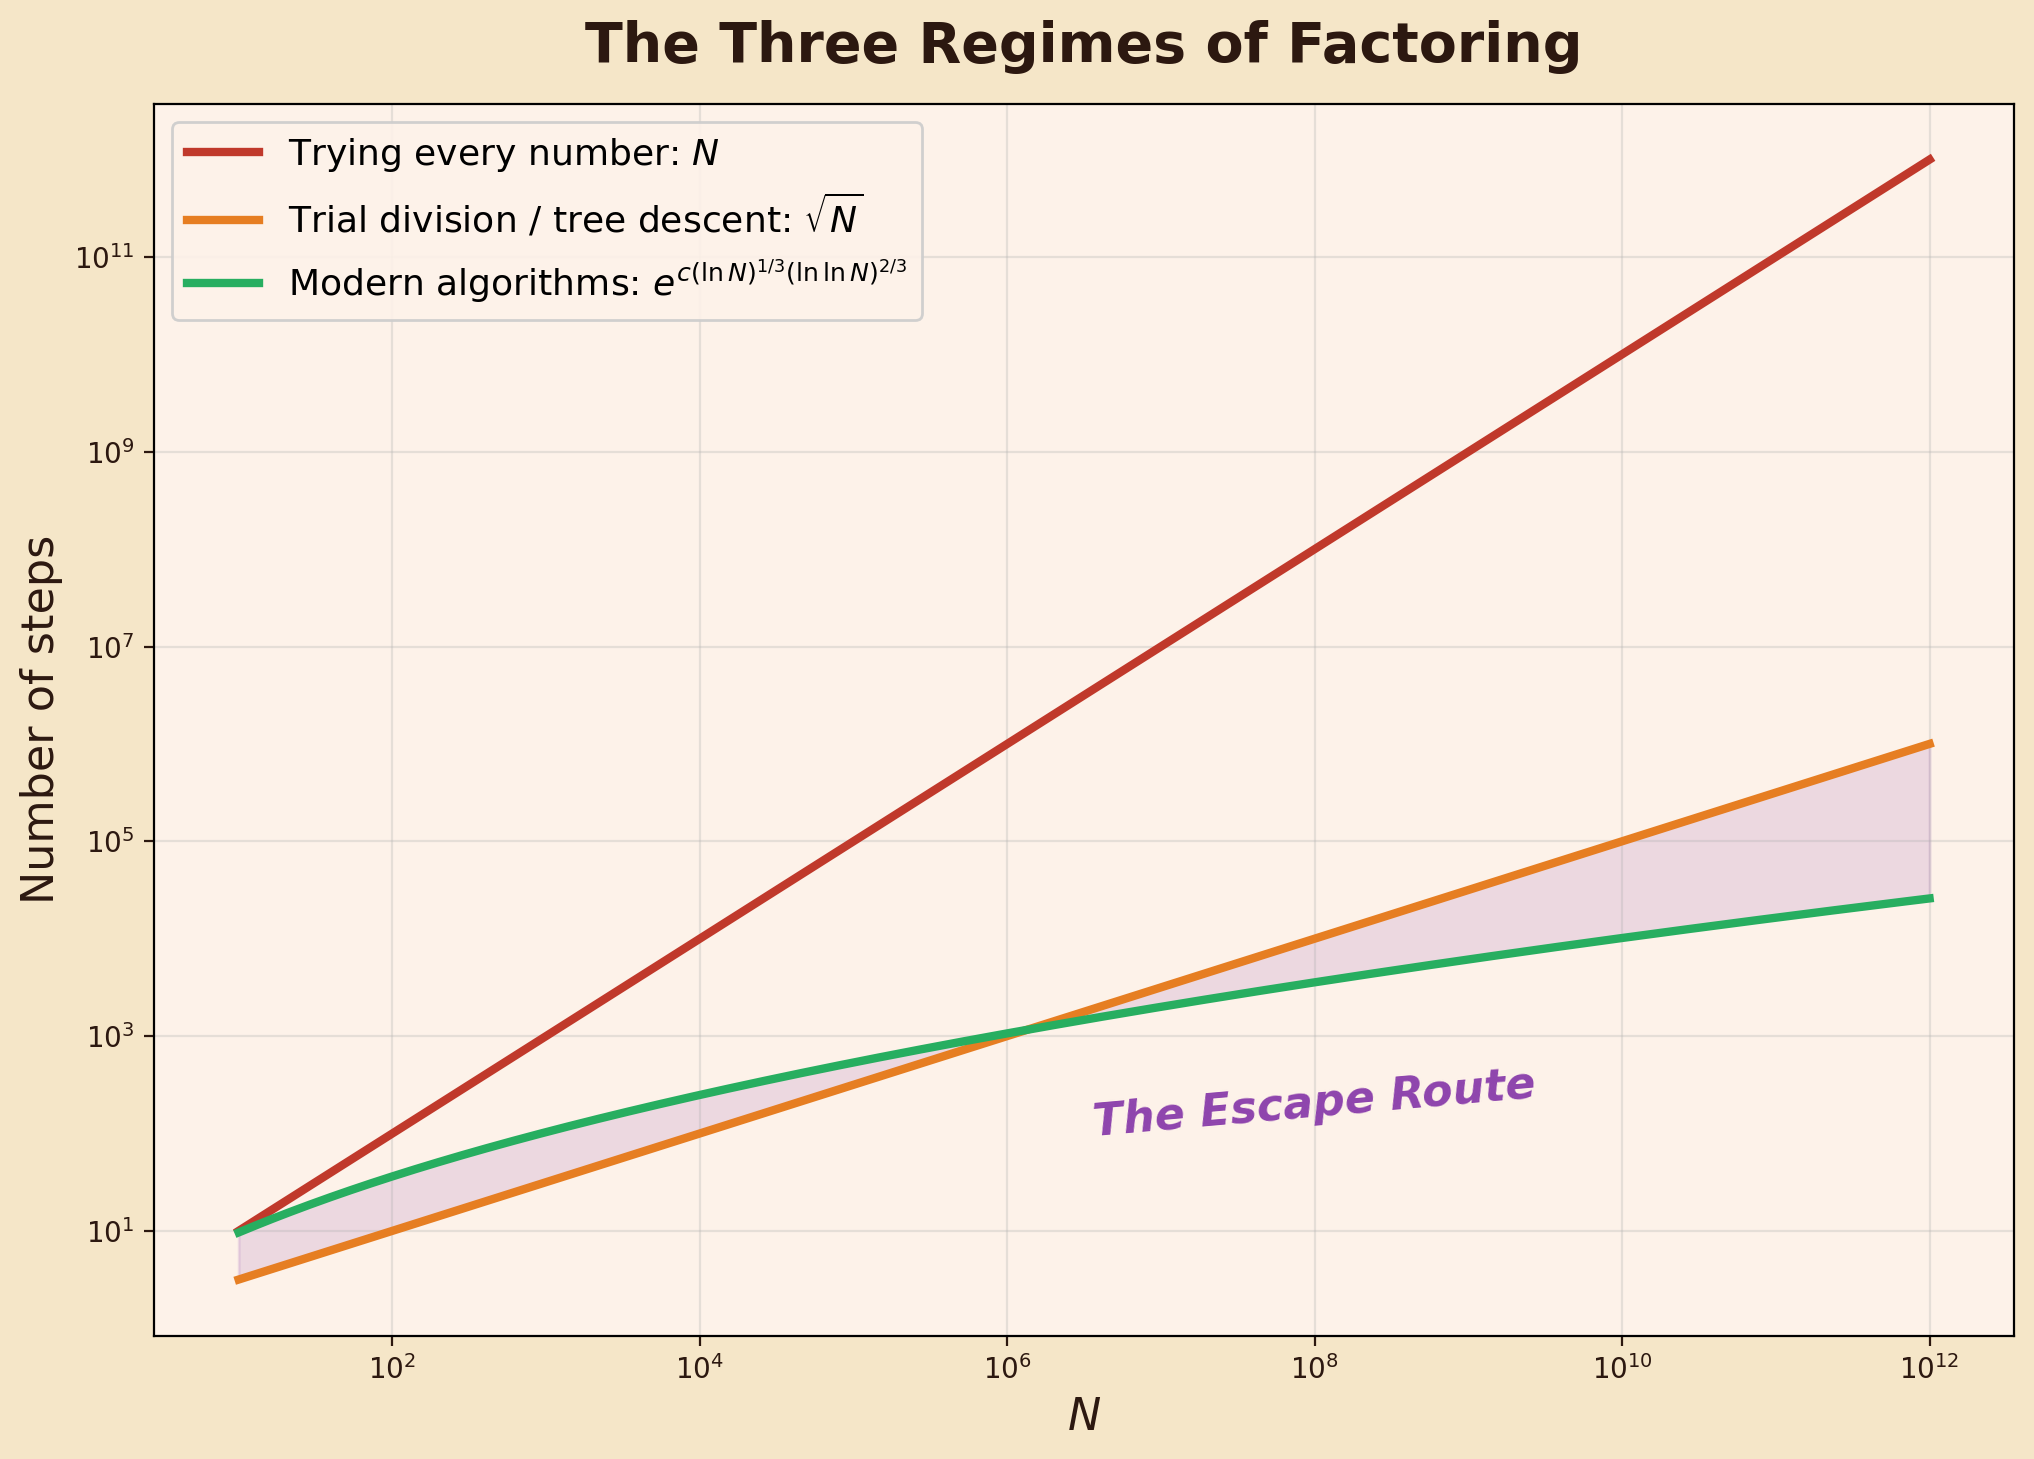
\includegraphics[width=0.82\textwidth]{../Chapter2/images/fig05_complexity_graph.png}
\end{figure}


The drama of integer factorization --- the problem that secures every online bank transaction, every encrypted email, every digital signature --- rests on this gap between \(\sqrt{N}\) and the sub-exponential algorithms that can actually crack large semiprimes. We will explore those algorithms in later chapters. For now, the lesson is clear: the Berggren tree is beautiful, but it is a two-dimensional creature, and two dimensions are not enough.



\section{Gauss and the Shortest Vector}\label{ch2-gauss-and-the-shortest-vector}

Carl Friedrich Gauss, at the age of nineteen, asked himself a question that sounds almost childishly simple. Imagine a parallelogram-shaped grid of dots extending to infinity in all directions --- a \emph{lattice}, in the mathematical sense. Each dot is obtained by taking some whole-number combination of two fixed ``basis'' vectors \(\mathbf{v}_1\) and \(\mathbf{v}_2\). The lattice is the set

\[
\Lambda = \{a\,\mathbf{v}_1 + b\,\mathbf{v}_2 : a, b \in \mathbb{Z}\}.
\]

Gauss's question: \emph{what is the shortest nonzero vector in this lattice?}

For a square grid --- \(\mathbf{v}_1 = (1, 0)\) and \(\mathbf{v}_2 = (0, 1)\) --- the answer is obvious: any of the four unit vectors \((1,0)\), \((-1,0)\), \((0,1)\), \((0,-1)\), each of length \(1\). But for a skewed lattice with basis vectors like \(\mathbf{v}_1 = (17, 0)\) and \(\mathbf{v}_2 = (5, 1)\), the shortest vector is far from obvious. It could be a complicated combination like \(2\mathbf{v}_1 - 7\mathbf{v}_2 = (34 - 35,\; 0 - 7) = (-1, -7)\), with length \(\sqrt{50} \approx 7.07\). Finding it requires \emph{reducing} the basis --- replacing the given (possibly bad) basis vectors with shorter, more orthogonal ones.

And here is Gauss's lovely insight: in two dimensions, the reduction algorithm is nothing other than the Euclidean algorithm. You repeatedly subtract multiples of the shorter vector from the longer one, just as the Euclidean algorithm subtracts multiples of the smaller number from the larger. After finitely many steps, you arrive at a \emph{reduced basis} --- a pair of vectors that are as short and as close to perpendicular as the lattice geometry allows. The shortest vector in the lattice is then simply the shorter of the two basis vectors.


\begin{figure}[htbp]
\centering
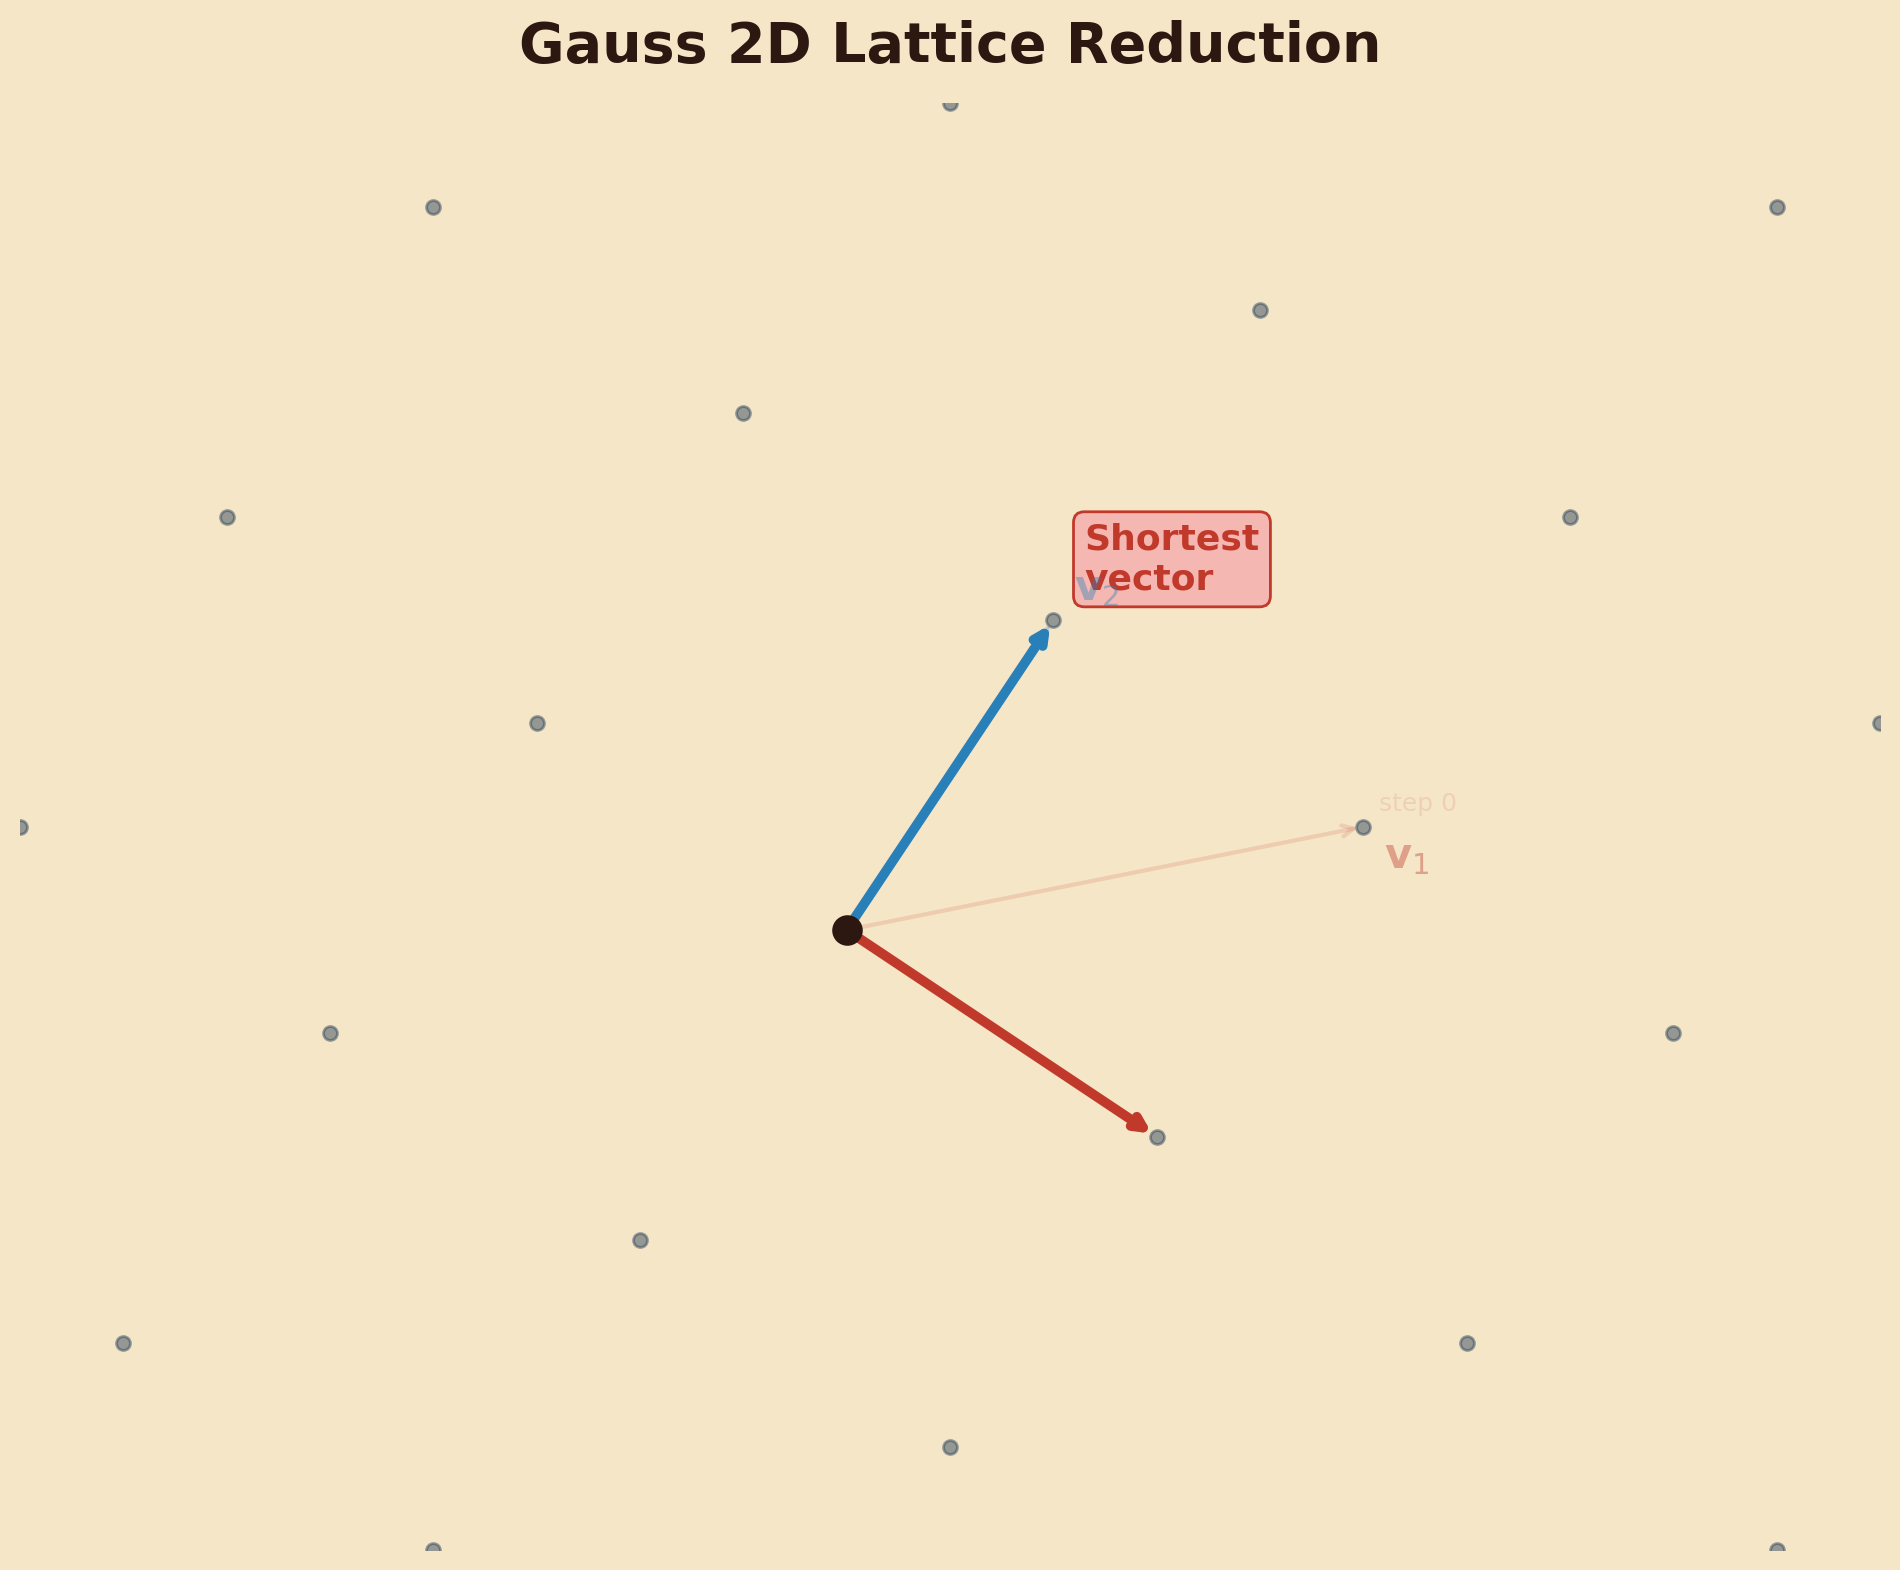
\includegraphics[width=0.82\textwidth]{../Chapter2/images/fig06_gauss_reduction.png}
\end{figure}


A key fact underpins this entire story, and it is worth stating carefully: for any two positive integers \(a\) and \(b\),

\[
\gcd(a, b) \le \min(a, b).
\]

Why? Because \(\gcd(a, b)\) divides both \(a\) and \(b\), and a positive divisor of a positive integer cannot exceed it. This seemingly trivial inequality is the foundation of the Euclidean algorithm's correctness: the remainders form a strictly decreasing sequence of positive integers, and such a sequence must terminate.

In the language of \index{lattice reduction}lattice reduction: the Euclidean algorithm finds the shortest vector in a two-dimensional lattice, and it does so \emph{optimally}. There is no cleverer algorithm, no shortcut, no trick that can do better in two dimensions. Gauss solved the problem completely.

Gauss published these ideas --- in the language of \emph{binary \index{quadratic form}quadratic forms} rather than lattices --- in his \emph{Disquisitiones Arithmeticae} of 1801, one of the most influential books in the history of mathematics. He was twenty-four. The ``reduction of binary quadratic forms'' that fills several chapters of the \emph{Disquisitiones} is, when you strip away the nineteenth-century notation, exactly the same algorithm we have been discussing: repeated subtraction of multiples, always choosing the best quotient, always driving the basis vectors shorter and more orthogonal. It would be another century and a half before anyone used the word ``lattice'' in this context, but Gauss had the substance, if not the terminology.

The connection to our story is now complete. The Berggren tree descent is the Euclidean algorithm. The Euclidean algorithm is Gauss's two-dimensional lattice reduction. Therefore, the Berggren tree is an \emph{optimal} lattice reduction algorithm in two dimensions. It is the best you can possibly do.



\section{The Wall at Two Dimensions}\label{ch2-the-wall-at-two-dimensions}

We have now proved something wonderful and something terrible at the same time.

The wonderful part: the Berggren tree is a perfect machine. It enumerates every primitive Pythagorean triple, it runs in reverse without jamming, and its descent algorithm is \emph{identical} to the best possible lattice reduction in two dimensions. There is a deep and beautiful correspondence --- the Lattice-Tree Correspondence --- linking a family tree of right triangles to the oldest algorithm in mathematics.

The terrible part: ``best possible in two dimensions'' means \(\Theta(\sqrt{N})\) for factoring. And for a \(300\)-digit number, \(\sqrt{N}\) has \(150\) digits. You would need more steps than there are atoms in the observable universe. The perfection of the machine is precisely what makes it useless for the hardest problems.

Let us be precise about what we have shown:

\begin{enumerate}
\def\labelenumi{\arabic{enumi}.}

\item
  The tree descent is the Euclidean algorithm (by the Lattice-Tree Correspondence).
\item
  The Euclidean algorithm is Gauss's lattice reduction in two dimensions (by inspection of the matrix operations).
\item
  Gauss's reduction in 2D is provably optimal (the shortest vector is found exactly).
\item
  Therefore, \emph{no trick within the two-dimensional framework can beat \(\Theta(\sqrt{N})\) for factoring}.
\end{enumerate}

This is not a failure of imagination. It is not that we have been insufficiently clever. It is a genuine \emph{impossibility result}: the two-dimensional approach has a hard ceiling, and no amount of ingenuity can break through it. The wall is made of mathematics, not of engineering, and mathematics does not negotiate.


\begin{figure}[htbp]
\centering
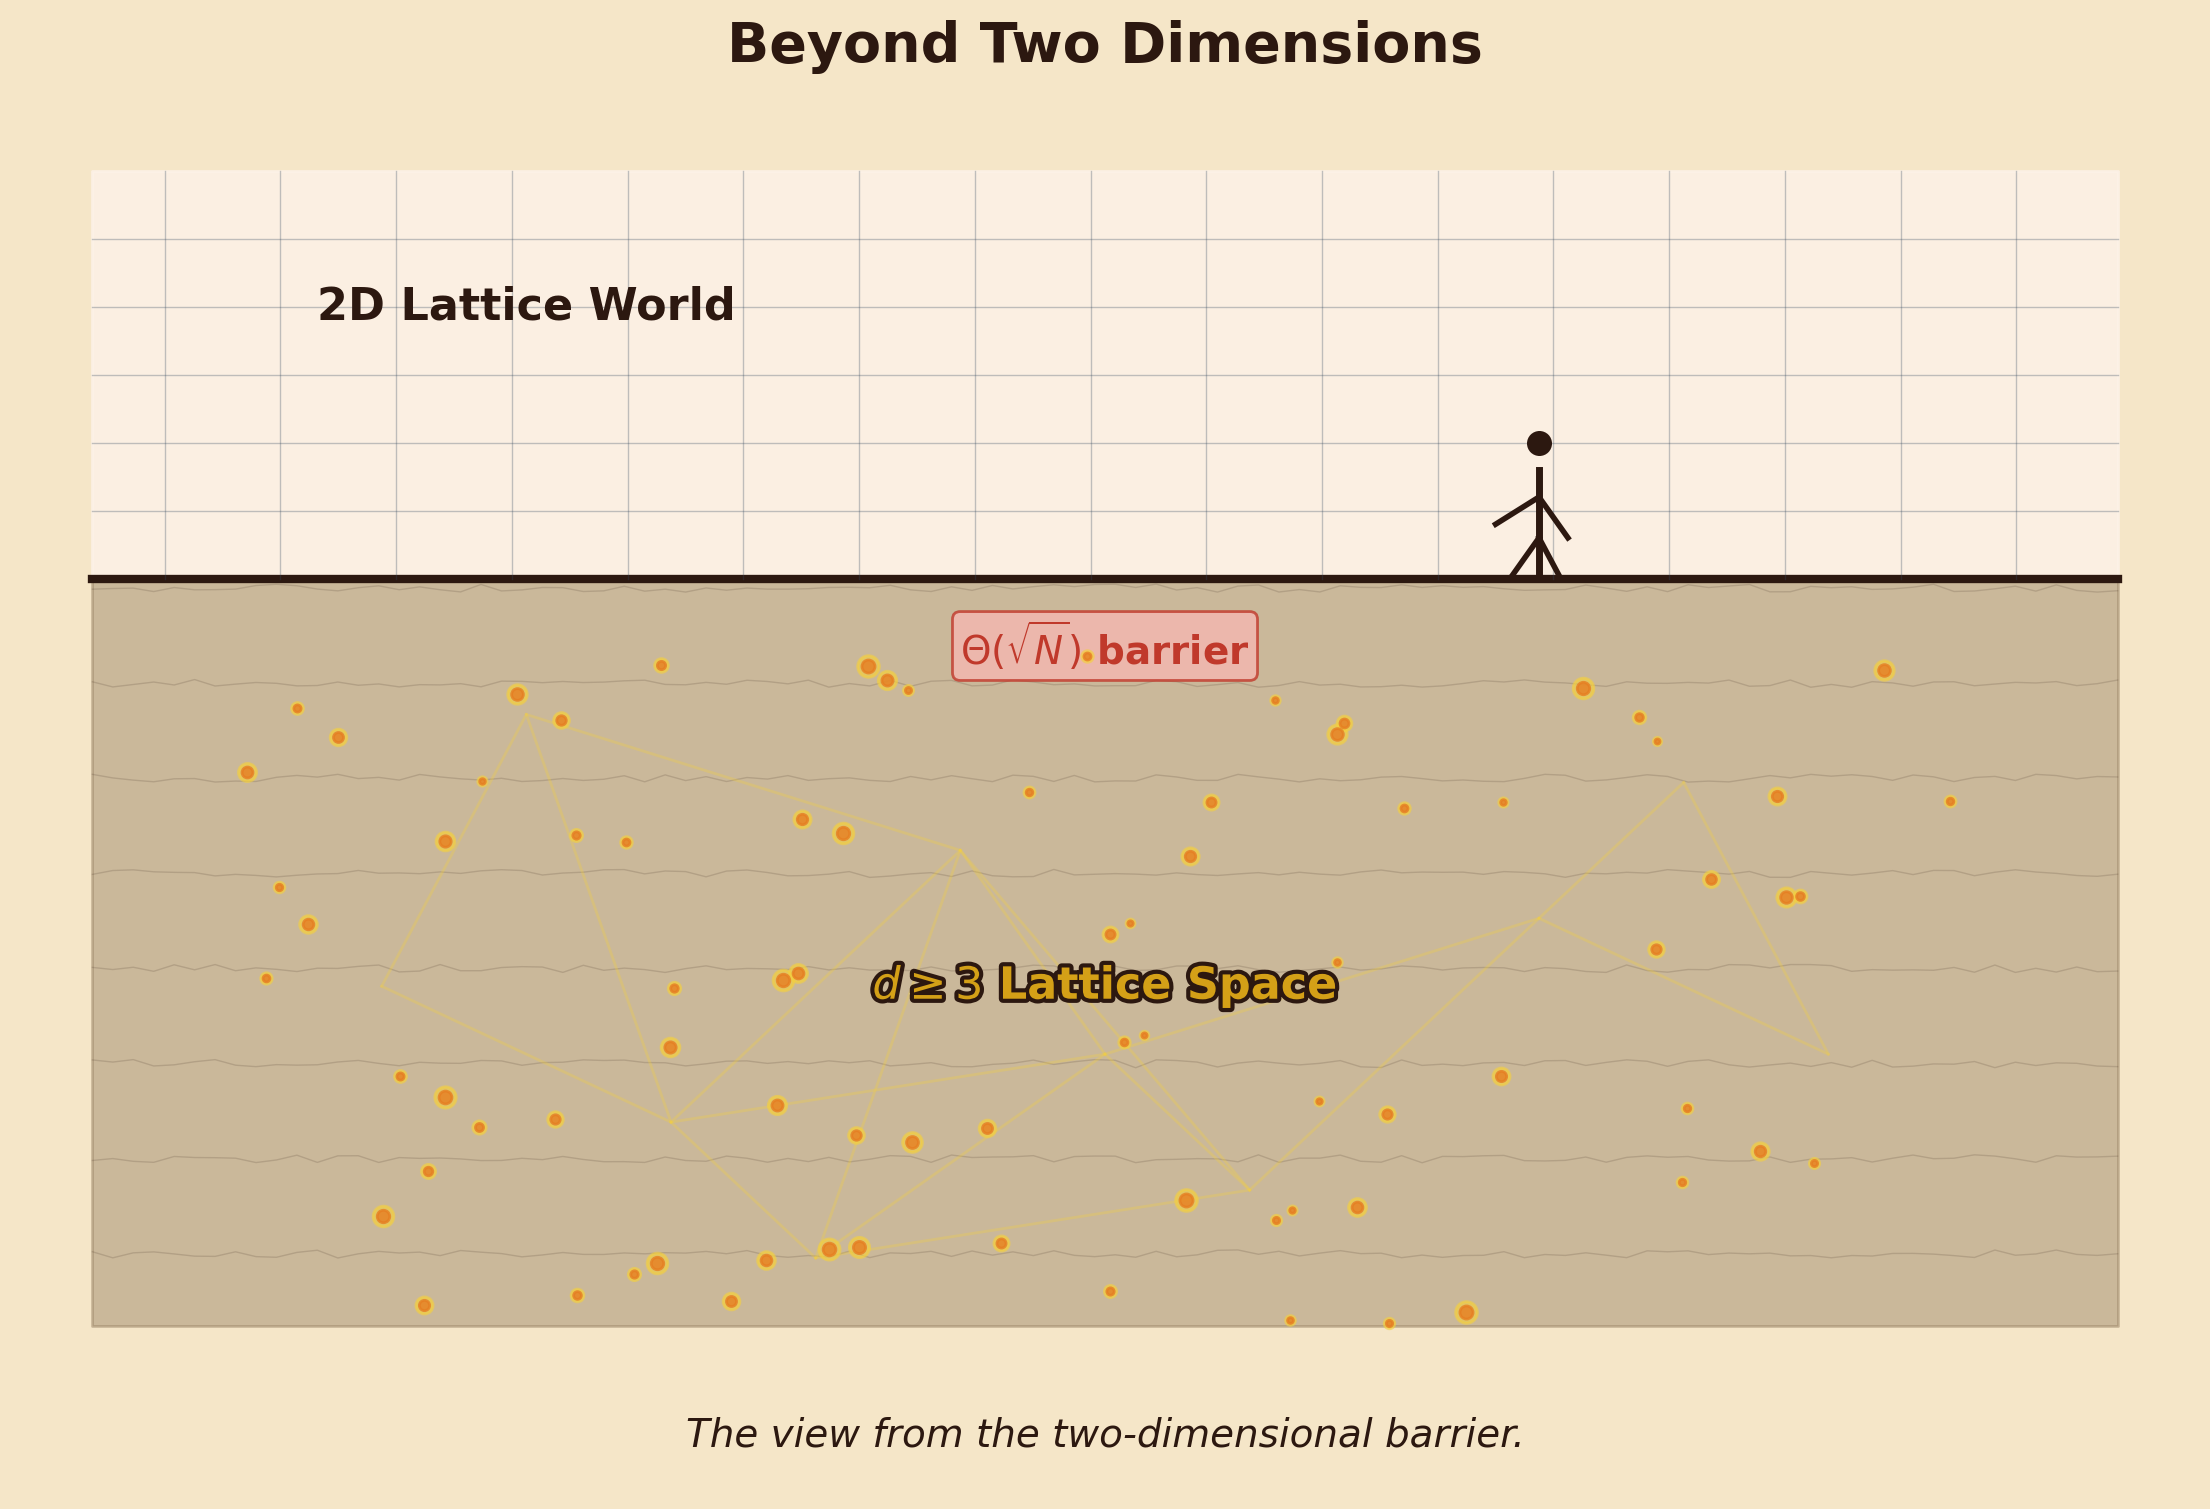
\includegraphics[width=0.82\textwidth]{../Chapter2/images/fig07_2d_barrier.png}
\end{figure}


Impossibility results have a distinguished history. In 1824, Abel proved that no formula involving radicals can solve the general quintic equation --- closing a quest that had consumed algebraists for three centuries. In 1931, Gödel proved that no consistent formal system powerful enough to express arithmetic can prove its own consistency --- shattering Hilbert's dream of a complete foundation for mathematics. In 1936, Turing proved that no algorithm can decide, for an arbitrary program, whether it will halt --- killing the \emph{Entscheidungsproblem} that Hilbert had posed in 1928. Each of these impossibility results was, at first, a disappointment. But each one was also a \emph{liberation}: by proving that a certain path leads nowhere, you free yourself to look for a different path entirely.

Our impossibility result is modest by comparison, but its message is the same. The two-dimensional framework --- Pythagorean triples, \(2 \times 2\) matrices, the Euclidean algorithm --- is a dead end for fast factoring. If we want to do better, we must escape Flatland.

The question becomes: \emph{what happens if we add a third dimension?}



\section{Through the Looking Glass: Higher Dimensions}\label{ch2-through-the-looking-glass-higher-dimensions}

In 1982, three mathematicians working in the Netherlands --- Arjen Lenstra, Hendrik Lenstra, and László Lovász --- discovered a way to break through the two-dimensional wall.

Their algorithm, known by their initials as LLL, does not find the \emph{shortest} vector in a lattice. (Finding the true shortest vector in high dimensions is NP-hard --- a problem widely believed to require exponential time in the worst case.) Instead, LLL finds a vector that is \emph{pretty short}: within a factor that depends on the dimension of the lattice. And ``pretty short,'' as it turns out, is short enough.

The LLL guarantee is this: in a lattice of dimension \(d\), the algorithm produces a nonzero vector whose length is at most \(2^{(d-1)/2}\) times the length of the true shortest vector. This factor is called the \emph{approximation ratio}. In two dimensions (\(d = 2\)), the factor is \(2^{1/2} = \sqrt{2} \approx 1.41\) --- practically exact. In three dimensions (\(d = 3\)), the factor is \(2^1 = 2\). In ten dimensions, the factor is \(2^{9/2} \approx 22.6\). In one hundred dimensions, the factor is \(2^{99/2} \approx 7.9 \times 10^{14}\) --- a huge number, but still \emph{finite}, and crucially, the algorithm runs in \emph{polynomial time}, meaning the number of arithmetic operations grows only as a polynomial in the dimension and the size of the input numbers.

The critical threshold is \(d = 3\). For \(d \ge 3\):

\[
\frac{d-1}{2} \ge 1 \implies 2^{(d-1)/2} \ge 2.
\]

In three or more dimensions, the approximation factor is at least \(2\). There is \emph{slack} --- the algorithm finds a vector that might be twice as long as the true shortest one, or longer. This slack is not a weakness. It is \emph{the mechanism} by which the algorithm achieves polynomial running time. Gauss's two-dimensional method finds the \emph{exact} shortest vector, but this perfection traps it in the two-dimensional world, where the factoring problem requires \(\Theta(\sqrt{N})\) time. LLL sacrifices perfection for speed, and the trade-off is spectacular: problems that would take the age of the universe in two dimensions become tractable in three or more.


\begin{figure}[htbp]
\centering
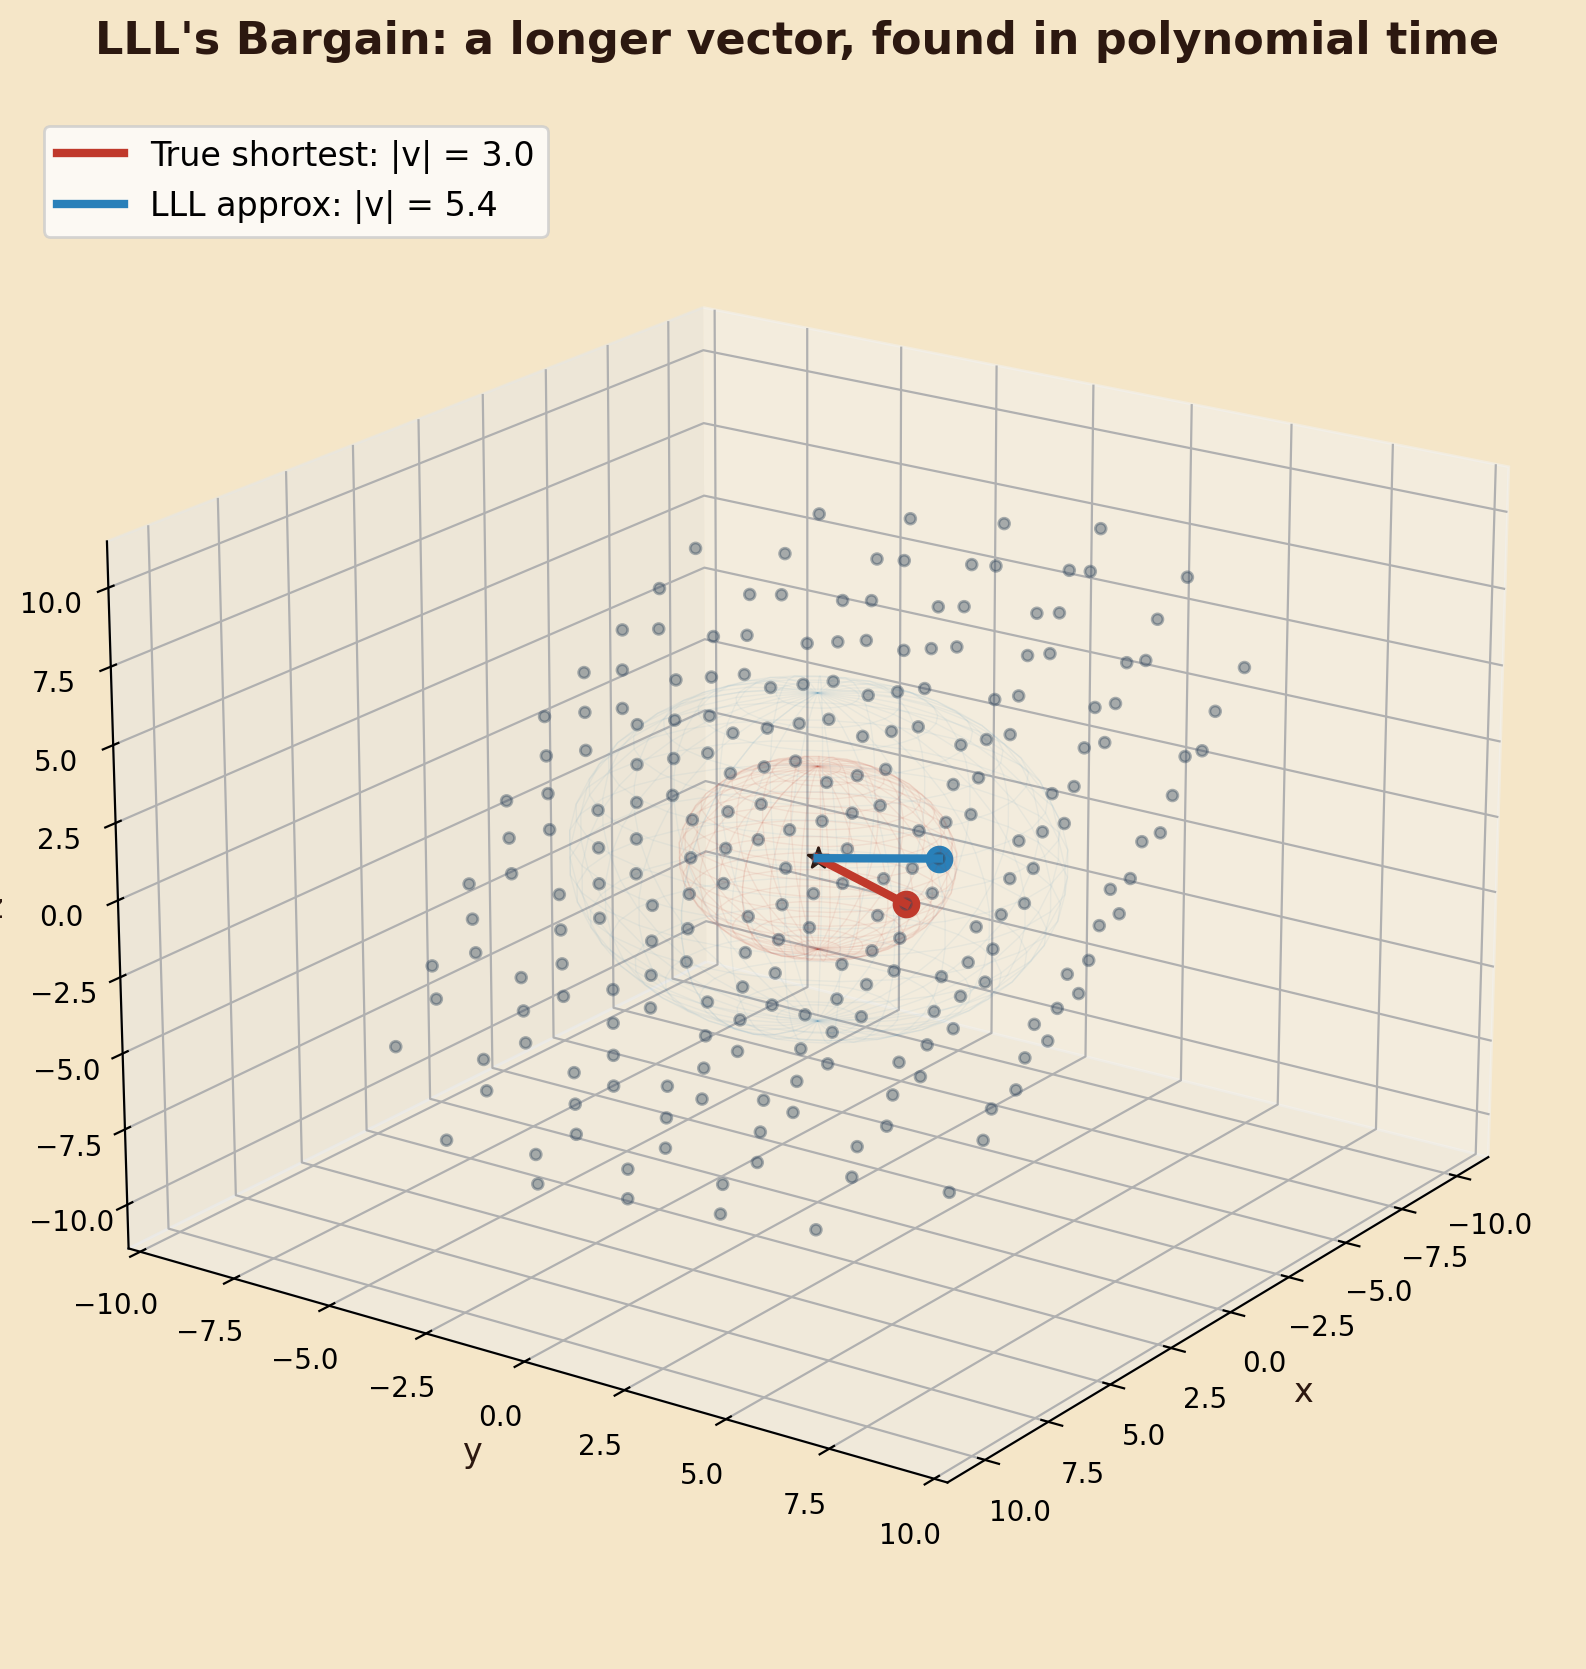
\includegraphics[width=0.82\textwidth]{../Chapter2/images/fig08_lll_bargain.png}
\end{figure}


The story of LLL's discovery is one of the great tales of twentieth-century mathematics. Lenstra, Lenstra, and Lovász were originally trying to factor polynomials with rational coefficients --- a problem that sounds purely algebraic and far removed from geometry. But they realized that the problem could be \emph{embedded} in a lattice: the coefficients of the polynomial factors correspond to short vectors in a cleverly constructed lattice. Find a short vector, and you find a factor. Their lattice reduction algorithm --- LLL --- cracked the polynomial factoring problem wide open, and then proceeded to demolish a series of other problems that nobody had expected it to touch.

Within a year of its publication, LLL was used to break the \emph{Merkle-Hellman knapsack cryptosystem}, one of the first public-key encryption schemes ever proposed. The scheme was based on the assumption that a certain combinatorial problem --- the subset sum problem --- was hard. LLL showed that it was not, at least not in the form Merkle and Hellman had used. The cryptographic community was stunned. Lovász himself was reportedly surprised by how broadly useful the algorithm turned out to be: ``We expected it to be a technical tool for one specific problem,'' he later recalled. ``We did not expect it to become a general-purpose weapon.''

The relevance to our story is this: if we can \emph{embed} the factoring problem into a lattice of dimension three or higher, then LLL can attack it --- and potentially do so in polynomial time, shattering the \(\sqrt{N}\) barrier that the two-dimensional Berggren tree cannot overcome. The two-dimensional wall is real, but it is not the end of the road. It is a \emph{floor}, and above it stretches a vast, higher-dimensional space full of possibilities.



\section{The Quadruple Lattice}\label{ch2-the-quadruple-lattice}

Consider three whole numbers \(x\), \(y\), and \(z\). They are linked to a secret number \(N\) by a single equation:

\[
x^2 + y^2 + z^2 \equiv 0 \pmod{N^2}.
\]

Can you find such a triple? Of course you can --- \((0, 0, 0)\) works trivially, since \(0 + 0 + 0 = 0\), and zero is divisible by everything. A mathematical ``of course, but so what?''

The \emph{interesting} solutions are the nonzero ones --- the triples with small but positive entries, whose squared sum is a nonzero multiple of \(N^2\). These are the solutions that reveal the factors of \(N\). Why? Because if \(x^2 + y^2 + z^2 = k \cdot N^2\) for some small integer \(k\), then \(\gcd(x, N)\) (or \(\gcd(y, N)\), or \(\gcd(z, N)\)) is likely to be a nontrivial factor of \(N\) --- not \(1\) and not \(N\) itself, but something in between.

The set of all integer triples \((x, y, z)\) satisfying \(x^2 + y^2 + z^2 \equiv 0 \pmod{N^2}\) forms a \emph{lattice} --- a regular, repeating pattern in three-dimensional space, just like the two-dimensional dot grids we discussed earlier, but with an extra dimension. Finding a \emph{short} nonzero vector in this lattice is exactly the kind of problem that LLL was born to solve.


\begin{figure}[htbp]
\centering
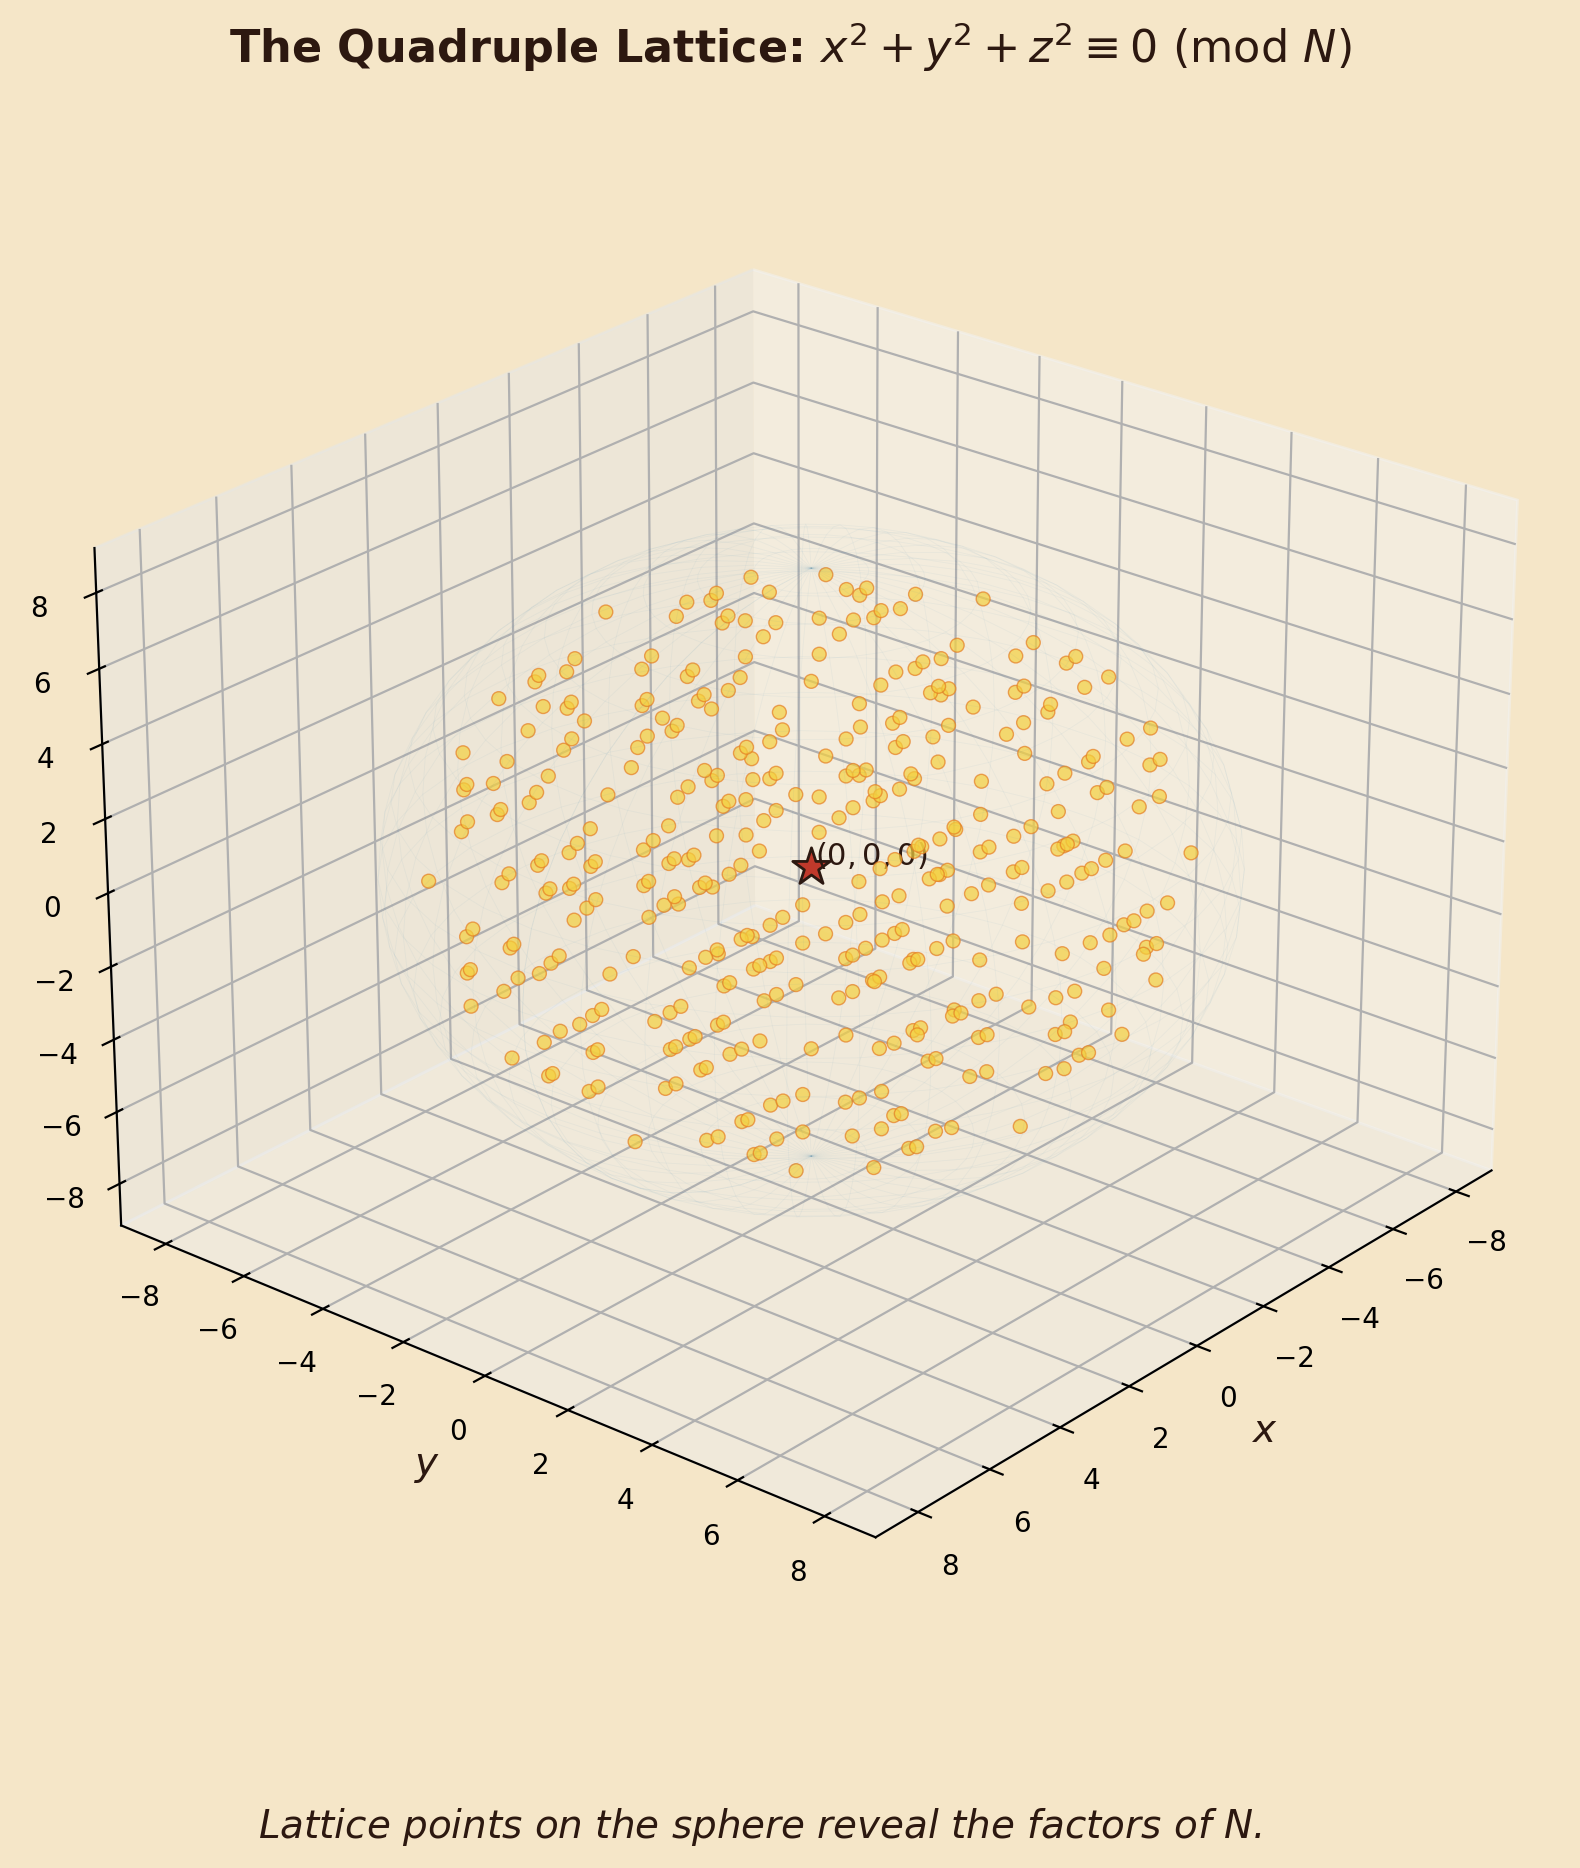
\includegraphics[width=0.82\textwidth]{../Chapter2/images/fig09_quadruple_lattice.png}
\end{figure}


We call this the \emph{quadruple lattice} --- a nod to the quadratic form \(x^2 + y^2 + z^2\) and to the algebraic structure it encodes. (The name also echoes the tradition of \emph{quadruple} representations in the theory of sums of squares, which stretches back through Jacobi and Lagrange to Fermat himself.)

The connection to our chapter's arc is now clear:

\begin{itemize}

\item
  In two dimensions, the Berggren tree and the Euclidean algorithm give us an optimal but slow method: \(\Theta(\sqrt{N})\).
\item
  In three dimensions, the quadruple lattice gives us a playing field where LLL can operate --- and LLL runs in polynomial time.
\item
  The Berggren tree was a beautiful dead end; the quadruple lattice is the door to the next room.
\end{itemize}

There is a deep and ancient tradition behind the idea of representing numbers as sums of squares. Fermat proved (in a letter on Christmas Day, 1640 --- hence ``Fermat's Christmas theorem'') that every prime of the form \(4k + 1\) can be written as a sum of two squares. Lagrange proved in 1770 that every positive integer is a sum of four squares. Jacobi found an exact formula for the \emph{number} of representations of \(n\) as a sum of four squares, involving the sum of the divisors of \(n\). These results are not merely ornamental --- they are the deep structural backbone that makes the quadruple lattice work. The solutions exist because the arithmetic of sums of squares has a rich algebraic structure, and that structure is precisely what we exploit when we embed the factoring problem into a lattice.



\section{The Map of the Journey}\label{ch2-the-map-of-the-journey}

Let us stand back and survey the landscape we have traversed.

We began with a toy factory --- two machines stamping out Pythagorean triples from a single seed. We discovered that these machines, with their integer entries and determinant one, belong to the special linear group \(\mathrm{SL}(2, \mathbb{Z})\), and that running them in reverse is always possible.

We then gave the Euclidean algorithm --- humanity's oldest nontrivial algorithm, at least 2,300 years old --- a makeover, writing each of its steps as multiplication by a \(2 \times 2\) quotient matrix. This let us see the algorithm as a \emph{path} through the space of all integer pairs, driven by a sequence of matrix multiplications.

And then came the astonishing coincidence: the inverse Berggren machines are Euclidean quotient matrices. Tracing a triple back through the tree to the root --- the tree descent --- performs the exact same computation as the Euclidean algorithm on the Euclid parameters \(m\) and \(n\). The tree \emph{is} the algorithm, wearing a disguise.

From there, the implications cascaded. The Euclidean algorithm is Gauss's lattice reduction in two dimensions. Gauss reduction in 2D is provably optimal. Therefore, no two-dimensional lattice method can beat \(\Theta(\sqrt{N})\) for factoring. The perfection of the Berggren tree is precisely what proves the limitation of the Berggren tree. It is the best you can do, and the best you can do is not enough.

But then --- the escape. In 1982, Lenstra, Lenstra, and Lovász showed that in three or more dimensions, lattice reduction can be performed in polynomial time, at the cost of finding approximately (rather than exactly) shortest vectors. The approximation factor \(2^{(d-1)/2}\) grows with the dimension, but the running time grows only polynomially. The slack in the approximation is the mechanism of the speed.

And finally, the quadruple lattice --- the three-dimensional arena where LLL can work its magic on the factoring problem. The two-dimensional wall is real, but it is not the end of the story. Above it stretches a vast higher-dimensional space, and in that space, algorithms exist that the two-dimensional world could never have dreamed of.


\begin{figure}[htbp]
\centering
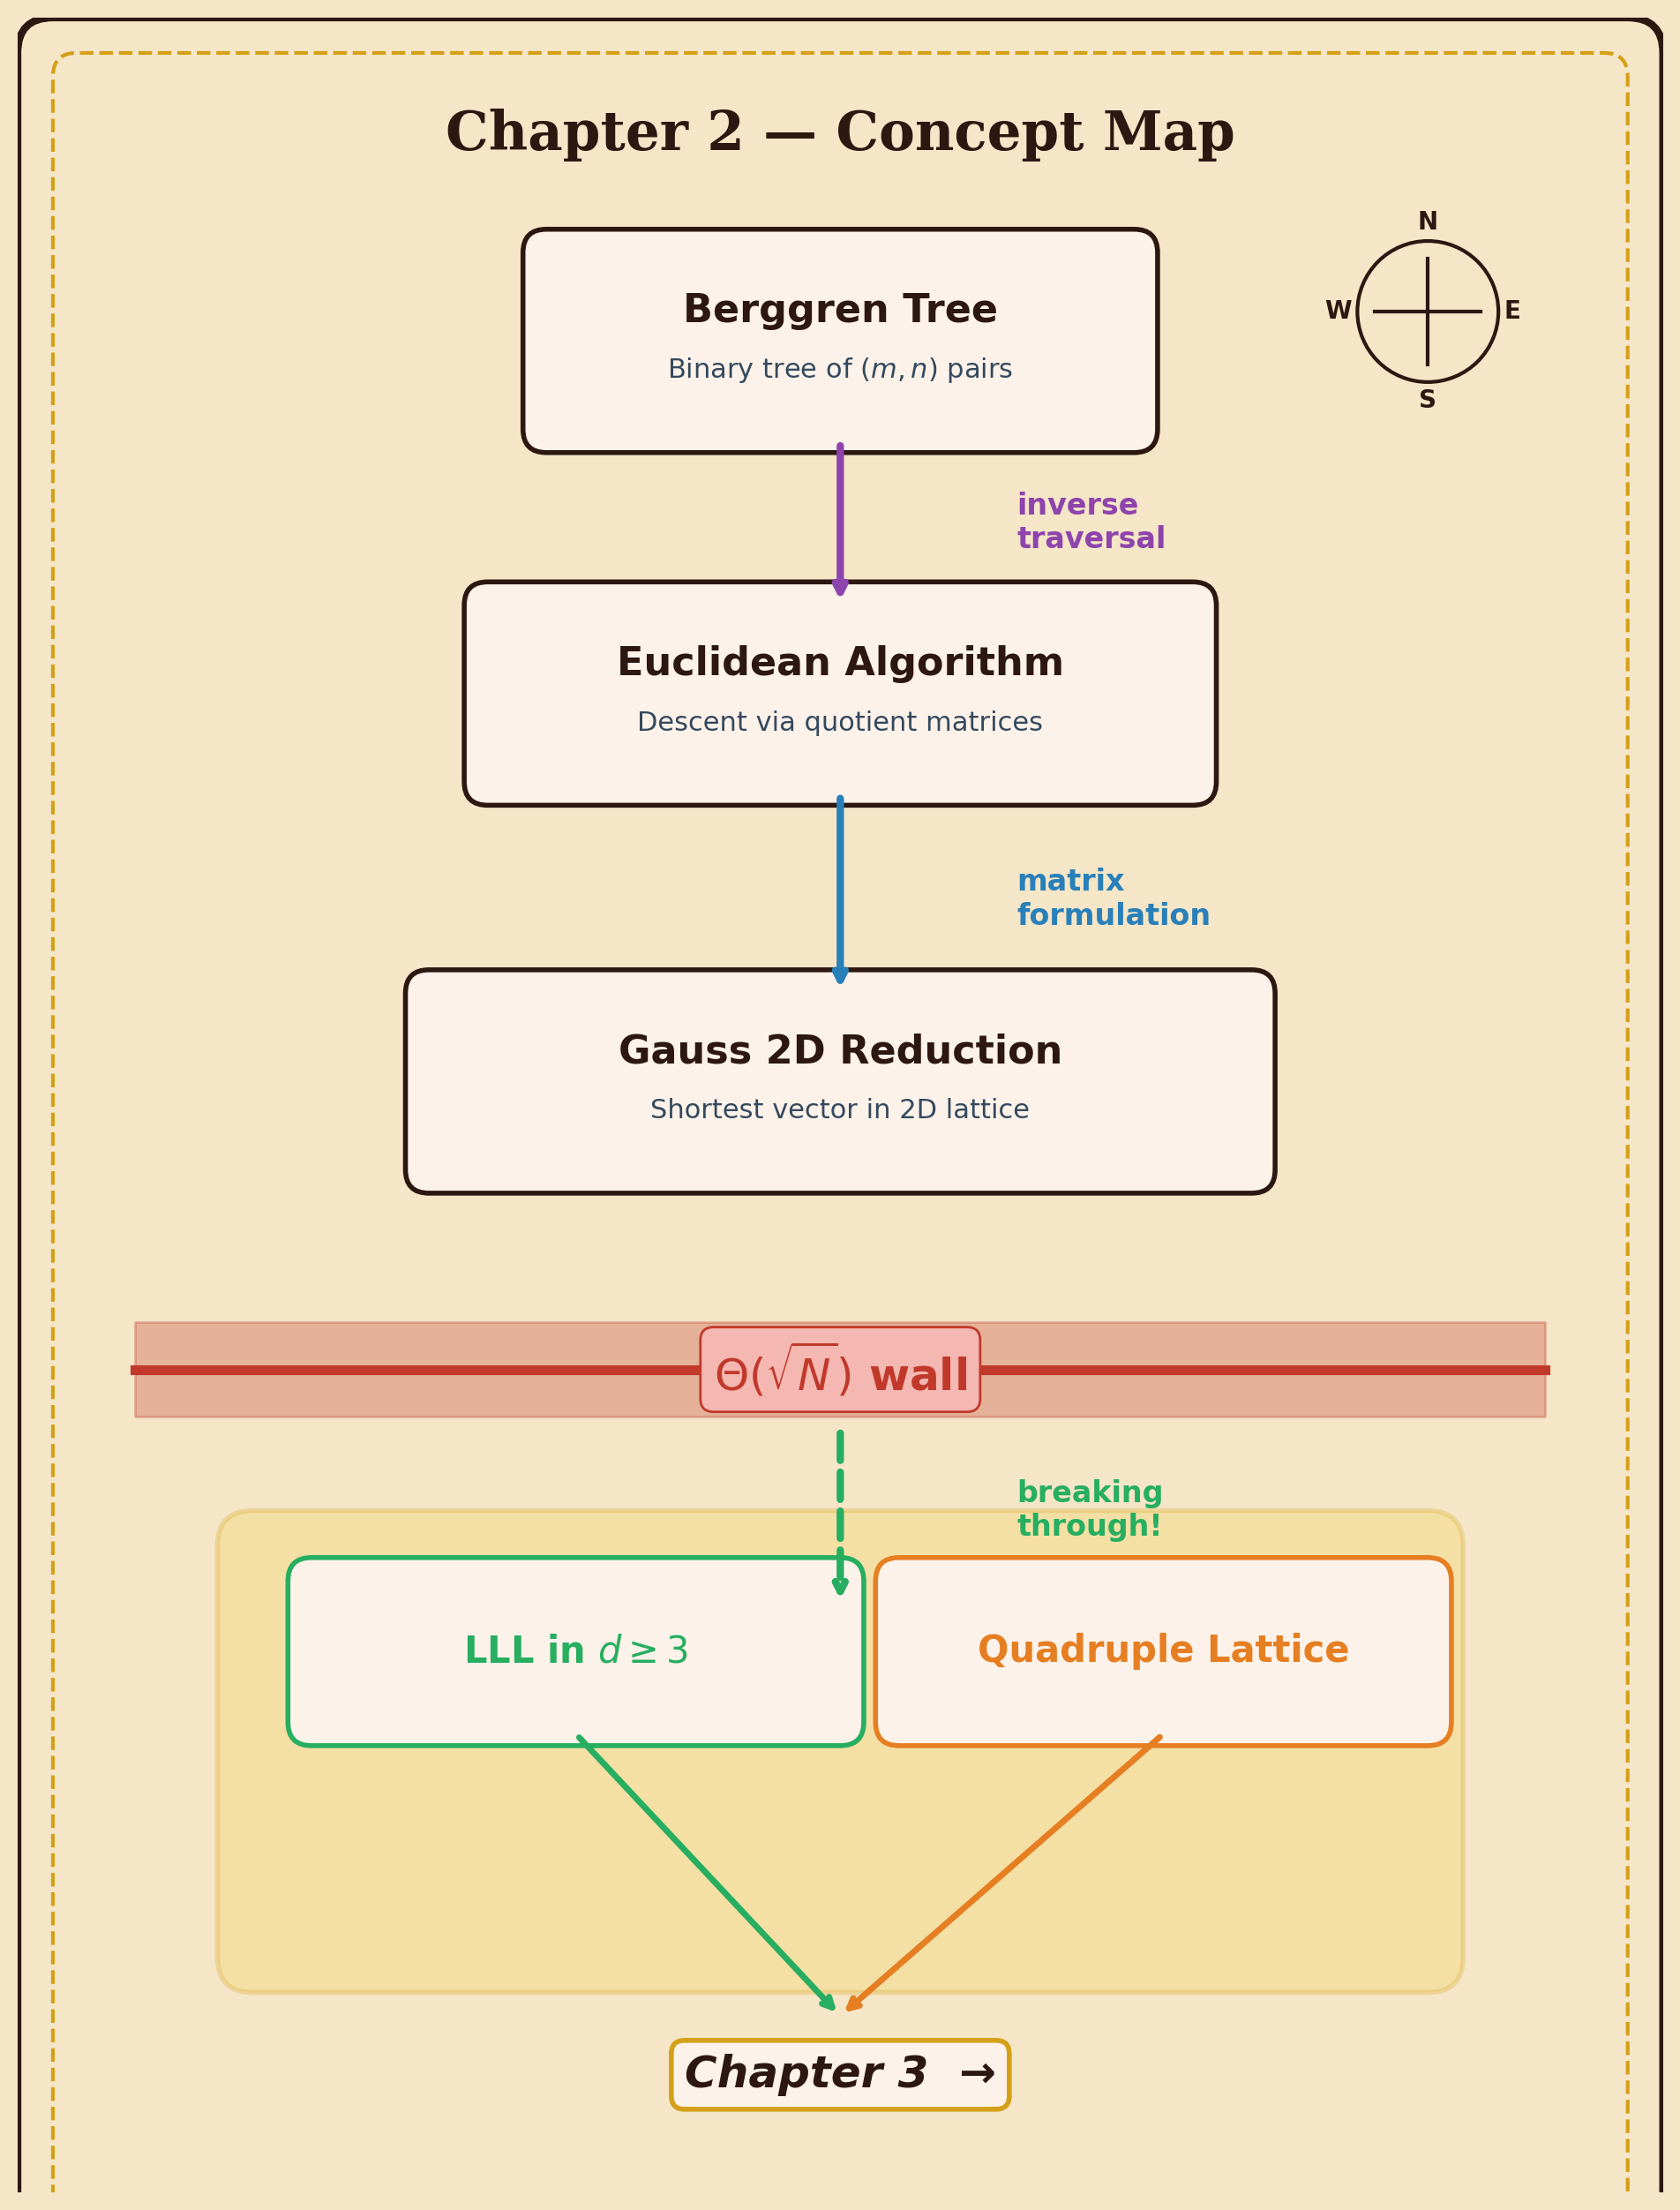
\includegraphics[width=0.82\textwidth]{../Chapter2/images/fig10_concept_map.png}
\end{figure}


There is a recurring theme in mathematics --- one of the grandest themes of all --- of \emph{seeing the same object from different angles}. The dozens of proofs of quadratic reciprocity, each illuminating a different facet of the same jewel. The Langlands program, which conjectures vast correspondences between number theory, geometry, and representation theory. The modularity theorem, which proved that elliptic curves and modular forms --- objects from seemingly unrelated branches of mathematics --- are secretly the same thing, and which, as a corollary, settled \index{Fermat's Last Theorem}Fermat's Last Theorem after 358 years. The Lattice-Tree Correspondence is a small but lovely instance of this grand pattern: the Berggren tree and the Euclidean algorithm are two faces of the same mathematical crystal, and recognizing their identity unlocks a precise understanding of what two-dimensional methods can and cannot do.

We have shown that the humble Pythagorean triple tree, for all its elegance, is secretly just one face of a much larger crystal. In two dimensions, we can see every facet perfectly --- but we cannot move. In three dimensions and beyond, the view is blurrier, but we are free to roam.

The next chapter will explore what happens when we actually start walking.



\section{Puzzles for the Reader}\label{ch2-puzzles-for-the-reader}

\begin{quote}
\textbf{Puzzle 1.} Apply \(\mathbf{M}_1\) and \(\mathbf{M}_3\) to the pair \((3, 2)\). What Pythagorean triples do the resulting pairs generate?
\end{quote}

\begin{quote}
\textbf{Puzzle 2.} Verify that \(\mathbf{M}_3^{-1} \cdot \mathbf{M}_3 = \mathbf{I}\) by direct matrix multiplication.
\end{quote}

\begin{quote}
\textbf{Puzzle 3.} Run the Euclidean algorithm on \((19, 7)\). Write each step as a quotient matrix \(\mathbf{Q}(q)\) and express the full computation as a matrix product.
\end{quote}

\begin{quote}
\textbf{Puzzle 4.} Starting from the pair \((m, n) = (9, 2)\), descend the Berggren tree to the root \((2, 1)\) by applying inverse machines. At each step, state which inverse machine you used and verify that the result matches a step of the Euclidean algorithm on \((9, 2)\).
\end{quote}

\begin{quote}
\textbf{Puzzle 5.} If \(N = 15 = 3 \times 5\), verify that \(p = 3 \le \sqrt{15} \approx 3.87\). How many trial divisions would it take to find the factor \(3\)?
\end{quote}

\begin{quote}
\textbf{Puzzle 6.} The LLL approximation factor in dimension \(d = 4\) is \(2^{3/2} = 2\sqrt{2} \approx 2.83\). In dimension \(d = 10\), it is \(2^{9/2} \approx 22.6\). At what dimension does the factor first exceed \(1000\)?
\end{quote}
